%%%%%%%%%%%%%%%%%%%%%%%%%%%%%%%%%%%%%%%%%%%%%%%%%%
%  JASA LaTeX Template File
%  To make articles using JASA.cls, Version 1.1
%  September 14, 2019
%%%%%%%%%%%%%%%%%%%%%%%%%%%%%%%%%%%%%%%%%%%%%%%%%%

%% Step 1:
%% Uncomment the style that you want to use:

%%%%%%% For Preprint
%% For manuscript, 12pt, one column style

\documentclass[preprint]{JASA}

%%%%% Preprint Options %%%%%
%% The track changes option allows you to mark changes
%% and will produce a list of changes, their line number
%% and page number at the end of the article.
%\documentclass[preprint,trackchanges]{JASA}


%% NumberedRefs is used for numbered bibliography and citations.
%% Default is Author-Year style.
%% \documentclass[preprint,NumberedRefs]{JASA}

%%%%%%% For Reprint
%% For appearance of finished article; 2 columns, 10 pt fonts

% \documentclass[reprint]{JASA}

%%%%% Reprint Options %%%%%

%% For testing to see if author has exceeded page length request, use 12pt option
%\documentclass[reprint,12pt]{JASA}


%% NumberedRefs is used for numbered bibliography and citations.
%% Default is Author-Year style.
% \documentclass[reprint,NumberedRefs]{JASA}

%% TurnOnLineNumbers
%% Make lines be numbered in reprint style:
% \documentclass[reprint,TurnOnLineNumbers]{JASA}

\usepackage{natbib}




% tightlist command for lists without linebreak
\providecommand{\tightlist}{%
  \setlength{\itemsep}{0pt}\setlength{\parskip}{0pt}}

% From pandoc table feature
\usepackage{longtable,booktabs,array}
\usepackage{calc} % for calculating minipage widths
% Correct order of tables after \paragraph or \subparagraph
\usepackage{etoolbox}
\makeatletter
\patchcmd\longtable{\par}{\if@noskipsec\mbox{}\fi\par}{}{}
\makeatother
% Allow footnotes in longtable head/foot
\IfFileExists{footnotehyper.sty}{\usepackage{footnotehyper}}{\usepackage{footnote}}
\makesavenoteenv{longtable}



\usepackage{tikz}
\usetikzlibrary{bayesnet}
% rotating must be loaded before tablefootnote
% \usepackage{rotating}
\usepackage{multirow}
\usepackage{colortbl}
\usepackage{tablefootnote}
\usepackage{amssymb}
\usepackage[caption=false]{subfig}
\usepackage{setspace}

\usepackage{fontspec}

%% Special font for IPA
%% Make sure "Doulos SIL" is installed on your computer
%% For other typefaces supporting IPA symbols, see
%% https://en.wikipedia.org/wiki/International_Phonetic_Alphabet#Typefaces
\newfontfamily\ipa{Doulos SIL} % Font for IPA symbols
\DeclareTextFontCommand{\ipatext}{\ipa}

%%%         Section for CJK Characters                   %%%
%%%   You may want to uncomment the code below if        %%%
%%%   you're writing this document with CJK characters   %%%

%\usepackage{xeCJK}  % Uncomment for using CJK characters
%% Set main font for CJK characters
%% Make sure your system has the font set
%\setCJKmainfont[
%	BoldFont={HanWangHeiHeavy}  % Set font for CJK boldface
%    ]{標楷體}    % Set font for normal CJK
%% Some Traditional Chinese fonts: AR PL KaitiM Big5, PingFang TC, Noto Sans CJK TC
%\XeTeXlinebreaklocale "zh"
%\XeTeXlinebreakskip = 0pt plus 1pt

%% Added by Florian to make biblatex and its \refsection work since pandoc does not parse 
%% content within latex environments. \refsection in turn is required to allow authors
%% to have multiple separate bibliographies (here: one for main text and one for SI).
%%
%% For some reasons it does seem to be necessary to reload the bibpackage here since
%% ---at least for my system---adding the following to the YAML header instead does
%% not seem to work:
%%
%%    biblio-style: apa
%%    biblatexoptions: [backend=biber,maxbibnames=999,style=apa]
%% 
%% curiously removing the following from the YAML header:
%%
%%     citation_package: biblatex
%%
%% makes knitr (or pandoc?) revert back to the default bibtex treatment, which does 
%% not allow multiple bibliographies.
% \usepackage[backend=biber, maxbibnames=999, style=apa]{biblatex}
% \addbibresource{latex-stuff/library.bib}
% \newcommand{\brefsection}{\begin{refsection}}
% \newcommand{\erefsection}{\end{refsection}}

\newcommand{\changelocaltocdepth}[1]{%
  \addtocontents{toc}{\protect\setcounter{tocdepth}{#1}}%
  \setcounter{tocdepth}{#1}%
}
\setcounter{tocdepth}{-10}
\changelocaltocdepth{-10}

\begin{document}
%% the square bracket argument will send term to running head in
%% preprint, or running foot in reprint style.

\title[Comparing normalization against perception]{Comparing accounts of formant normalization against US English listeners' vowel perception}

% ie
%\title[JASA/Sample JASA Article]{Sample JASA Article}

%% repeat as needed

\author{Anna Persson}
% ie
%\affiliation{Department1,  University1, City, State ZipCode, Country}
\affiliation{Swedish Language and Multilingualism, Stockholm University}
%% for corresponding author
\email{anna.persson@su.se}
%% for additional information

\author{Santiago Barreda}
% ie
%\affiliation{Department1,  University1, City, State ZipCode, Country}
\affiliation{Linguistics, University of California, Davis}
%% for corresponding author

%% for additional information

\author{T. Florian Jaeger}
% ie
%\affiliation{Department1,  University1, City, State ZipCode, Country}
\affiliation{Brain and Cognitive Sciences, Data Science, University of Rochester}
%% for corresponding author

%% for additional information


% ie
% \author{Author Four}
% \email{author.four@university.edu}
% \thanks{Also at Another University, City, State ZipCode, Country.}

%% For preprint only,
%  optional, if you want want this message to appear in upper left corner of title page
\preprint{Persson, Barreda, \& Jaeger, JASA}

%ie
%\preprint{Author, JASA}

% optional, if desired:
%\date{\today}
\date{\today}

\begin{abstract}
% Put your abstract here. Abstracts are limited to 200 words for
% regular articles and 100 words for Letters to the Editor. Please no
% personal pronouns, also please do not use the words ``new'' and/or
% ``novel'' in the abstract. An article usually includes an abstract, a
% concise summary of the work covered at length in the main body of the
% article.
Human speech perception tends to achieve robust speech recognition, despite substantial cross-talker variability. Believed to be critical to this ability are auditory normalization mechanisms whereby listeners adapt to individual differences in vocal tract physiology in vowel perception. This study asks what types of computations are involved in such normalization. Two 8-way alternative forced-choice experiments assessed L1 listeners' categorizations across the entire US English vowel space---both for unaltered and for synthesized stimuli. Listeners' responses in these experiments were compared against the predictions of twenty influential normalization accounts that differ starkly in the inference and memory capacities they imply for speech perception. Listeners' responses were best explained by \emph{extrinsic} normalization accounts, suggesting that listeners learn and store distributional properties of talkers' speech. Of the extrinsic accounts, it was the \emph{computationally least complex} variants that best fit listeners' responses, using a single parameter. These findings have consequences for any research that aims to investigate the perceptual, social, and linguistic information of vowel productions. This includes research in phonetics and phonology, sociolinguistics, and language acquisition. In these fields, it remains common to employ normalization accounts that the present study confirms to be inadequate models of human perception (e.g., Lobanov normalization).
\end{abstract}

%% pacs numbers not used

\maketitle

%  End of title page for Preprint option --------------------------------- %

%% See preprint.tex/.pdf or reprint.tex/.pdf for many examples


%  Body of the article
\setcounter{secnumdepth}{5}
\setcounter{page}{1}
\setcounter{section}{0}

\section{Introduction}\label{sec:intro}

One of the central challenges for speech perception originates in cross-talker variability: depending on the talker, the same acoustic signal can encode different sound categories \citep{allen2003, liberman1967, newman2001}. This results in ambiguity in the mapping from acoustics to words and meanings. Research has identified several mechanisms through which listeners resolve this ambiguity, ranging from early perceptual processes, to adaptation of phonetic categories, all the way to adjustments in post-linguistic decision processes \citep[for review, see][]{xie2023}. The present study focuses on the first type of mechanism, early auditory processes that transform and normalize the acoustic input into the perceptual cues that constitute the input to linguistic processing \citep[for reviews,][]{barreda2020, johnson-sjerps2021, mcmurray-jongman2011, stilp2020, weatherholtz-jaeger2016}. We seek to respond, in particular, to recent calls to put theories of adaptive speech perception to stronger tests \citep{baeseberk2018, schertz-clare2020, xie2023}.

Evidence for the presence of early normalization mechanisms comes from neuroimaging and neurophysiological studies \citep[e.g.,][]{oganian2023, skoe2021}. These studies have decoded effects of talker identity from subcortical brain areas like the brain stem, and thus prior to the cortical regions believed to encode linguistic categories \citep[e.g.,][]{sjerps2019, tang2017}. This includes brain responses that lag the acoustic signal by as little as 20-50 msecs \citep{lee2009}, suggesting very fast and highly automatic processes. By removing talker-specific variability from the phonetic signal early, auditory normalization offers elegant and effective solutions to cross-talker variability, that might reduce the need for more complex adaptation of individual phonetic categories further upstream \citep{apfelbaum-mcmurray2015, xie2023}.\footnote{Normalization does not necessarily imply that \emph{only} talker-normalized auditory percepts are available to subsequent processing. There is ample evidence that subcategorical information can enter listeners' representations of sound categories \citep[e.g.,][]{hay2017, hay2019, johnson1999, mcgowan2015, walker-hay2011}, in line with episodic \citep{goldinger1996} and exemplar theory of speech perception \citep{johnson1997, sumner2011}.}

While it is relatively uncontroversial \emph{that} normalization contributes to robust speech perception, it is still unclear what types of computations this implicates. We address this question for the perception of vowels, which cross-linguistically relies on peaks in the distribution of spectral energy over acoustic frequencies (formants). Vowel perception has long been a focus in research on normalization \citetext{\citealp[e.g.,][]{bladon1984}; \citealp{fant1975}; \citealp{gerstman1968}; \citealp{johnson2020}; \citealp{joos1948}; \citealp{lobanov1971}; \citealp{miller1989}; \citealp{nearey1978}; \citealp{nordstrom-lindblom1975}; \citealp{syrdal-gopal1986}; \citealp{traunmuller1981}; \citealp{watt-fabricius2002}; \citealp{zahorian-jagharghi1991}; \citealp[for review, see][]{barreda2020}}, with some reviews citing over 100 competing proposals \citep{carpenter-govindarajan1993}. Importantly, these accounts differ in the types and complexity of computations they assume to take place during normalization. On the lower end of computational complexity, comparatively simple static transformations of the acoustic signal might suffice to achieve invariance in the mapping from cues to phonetic categories. For example, there is evidence that a transformation of acoustic frequencies (measured in Hz) into the psycho-acoustic Mel-space better describes how listeners perceive differences in the frequency of sine tones \citetext{\citealp[e.g.,][]{fastl-zwicker2007}; \citealp{stevens-volkmann1940}; \citealp[for a critique, see][]{greenwood1997}; \citealp{siegel1965}}. It is thus possible that cross-talker variability in vowel pronunciations is effectively reduced when formants are represented in Mel, rather than Hz. Similar arguments have been made about other psycho-acoustic transformations \citetext{\citealp[e.g., Bark,][]{traunmuller1990}; \citealp[ERB,][]{glasberg-moore1990}; \citealp[or semitones,][]{fant2002}}. Most of these accounts share that they log-transform acoustic frequencies---in line with neurophysiological evidence that the auditory representations in the brain seem to follow a roughly logarithmic organization, so that auditory perception is (up to a point) more sensitive to differences between lower frequencies than to the same difference between higher frequencies \citetext{\citealp[e.g.,][]{merzenich1975}; \citealp[for review, see][]{saenz-langers2014}}. If such static psycho-acoustic transformations are sufficient for formant normalization, this would offer a particularly parsimonious account of vowel perception as listeners would not have to infer talker-specific properties.

The parsimony of psycho-acoustic transformations contrasts with the majority of accounts for vowel normalization, which introduce additional computations. This includes accounts that normalize formants relative to other information that is available at the same point in the acoustic signal \citep[intrinsic normalization, e.g.,][]{miller1989, peterson1961, syrdal-gopal1986}. For example, according to one proposal, listeners normalize vowel formants by the vowel's fundamental frequency or other formants estimated at the same point in time \citep{syrdal-gopal1986}. To the extent that the fundamental frequency is correlated with the talkers' vocal tract size \citep[for review, see][]{vorperian-kent2007}, this allows the removal of physiologically-conditioned cross-talker variability in formant realizations. While such intrinsic accounts arguably entail more computational complexity than static transformations, they do not require that listeners \emph{maintain} talker-specific estimates over time. This distinguishes intrinsic from extrinsic accounts, which introduce additional computational complexity.

According to extrinsic accounts, normalization mechanisms infer and store estimates of talker-specific properties that then are used to normalize subsequent speech from that talker \citetext{\citealp{gerstman1968}; \citealp{lobanov1971}; \citealp{nearey1978}; \citealp{nordstrom-lindblom1975}; \citealp{watt-fabricius2002}; \citealp[for review, see also][]{weatherholtz-jaeger2016}}. At the upper end of computational complexity, some accounts hold that listeners continuously infer and maintain both talker-specific means for each formant and talker-specific estimates of each formant's variability \citep{gerstman1968, lobanov1971}. These estimates are then used to normalize formants, e.g., by centering and standardizing them \citep[essentially z-scoring formants,][]{lobanov1971}, removing cross-talker variability in the distribution of formant values. There are, however, more parsimonious extrinsic accounts that require inference and maintenance of fewer talker-specific properties. The most parsimonious of these is Nearey's \emph{uniform scaling} account, which assumes that listeners infer and maintain a single talker-specific parameter. This parameter (\(\Psi\)) can be thought of as capturing the effects of the talkers' vocal tract length on the spectral scaling applied to the formant pattern produced by a talker \citep{nearey1978}.\footnote{Under uniform scaling accounts, listeners essentially `slide' the center of their category representations (e.g, the `template' of vowel categories for a given dialect) along a single line in formant space, with \(\Psi\) determining the target of this sliding. Later extensions of this account maintain its memory parsimony but increased its inference complexity by allowing both intrinsic (the current F0) and extrinsic information (the talker's single mean of log-transformed formants) to influence the inference of \(\Psi\) \citep{nearey-assmann2007}. We return to this extension in the general discussion.} Uniform scaling deserves particular mention here as it is arguably one of the most developed normalization accounts, and rooted in principled considerations about the physics of sound and the evolution of auditory systems \citep[for review, see][]{barreda2020}.

In summary, hypotheses about the computations implied by formant normalization differ in the flexibility they afford as well as the inference and memory complexity they entail. Considerations about the complexity of inferences---essentially the number of parameters that listeners are assumed to estimate at any given moment in time---arguably gain in importance in light of the speed at which normalization seems to unfold. In the present study, we thus ask whether computationally simple accounts are sufficient to explain human vowel perception.



\begin{figure}

{\centering \includegraphics[width=0.95\linewidth]{../../figures/knitted/two-talkers} 

}

\caption{Illustration of how height, which is positively correlated with vocal tract size, affects vowels' F1 and F2, and how normalization can partially remove this effect. Shown here are realizations of all 8 monophthong vowels of US English by a short (cyan) and a tall native talker (red). \textbf{Panel A:} In the acoustic space, prior to any normalization (Hz). \textbf{Panel B:} After uniform scaling \citep{nearey1978}. \textbf{Panel C:} After Lobanov normalization \citep{lobanov1971}. The present study compares three of these accounts, along with 17 other normalization accounts.}\label{fig:two-talkers}
\end{figure}

While previous research has compared normalization accounts across languages, most of this work has evaluated proposals in terms of how well the normalized phonetic space supports the separability of vowel categories \citep{adank2004, carpenter-govindarajan1993, cole2010, escudero-bion2007, johnson-sjerps2021, syrdal1985}. This approach is illustrated in Figure \ref{fig:two-talkers}. These studies have found that computationally more complex accounts---which also afford more flexibility---tend to achieve higher category separability and higher categorization accuracy \citep[for review, see][]{persson-jaeger2023}. This includes Lobanov normalization, which continues to be highly influential in, for example, variationist and sociolinguistic research because of its effectiveness in removing cross-talker variability \citep[for a critique, see][]{barreda2021}. It is, however, by no means clear that human speech perception employs the same computations that achieve the best category separability or accuracy \citep[see also discussion in][]{barreda2021, nearey-assmann2007}.

A substantially smaller body of research has addressed this question by comparing normalization accounts against \emph{listeners' perception} \citetext{\citealp{barreda-nearey2012}; \citealp{barreda2021}; \citealp{nearey1989}; \citealp{richter2017}; \citealp[for a review, see][]{whalen2016}}. Interestingly, these works seem to suggest that computationally simpler accounts might provide a better fit against human speech perception than the influential Lobanov model \citep{barreda2021, richter2017}. For example, \citet{barreda2021} compared the predictions of uniform scaling and Lobanov normalization against listeners' categorization responses in a forced-choice categorization task over parts of the US English vowel space. In his experiment, listeners' categorization responses were better predicted by uniform scaling than by Lobanov normalization. Findings like these suggest that comparatively simple corrections for vocal tract size---such as uniform scaling---might provide a better explanation of human perception than more computationally complex accounts \citep[see also][]{johnson2020, richter2017}.

This motivates the present work. We take a broad-coverage approach by comparing the 20 normalization accounts in Table \ref{tab:norm-accounts} against the perception of all 8 monophthongs of US English (\ipatext{[i]} as in \emph{heed}, \ipatext{[ɪ]} in \emph{hid}, \ipatext{[ɛ]} in \emph{head}, \ipatext{[æ]} in \emph{had}, \ipatext{[ʌ]} in \emph{hut}, \ipatext{[ʊ]} in \emph{hood}, \ipatext{[u]} in \emph{who'd}, \ipatext{[ɑ]} in \emph{odd}).\footnote{We use Johnson's (2020) implementation of \citet{nordstrom-lindblom1975}. We group both \citet{nordstrom-lindblom1975} and \citet{johnson2020} with the centering accounts, as they are essentially variants of uniform scaling, differing in their estimation of \(\Psi\). We also include both versions of Syrdal \& Gopal's Bark-distance model. The two versions differ only in their normalization of F2, and have not previously been compared against human perception.} We do so for the perception of both natural and synthesized speech. Our broad-coverage approach complements previous studies, which have typically compared a small number of accounts (up to 3) and focused on parts of the vowel inventory, and thus parts of the formant space \citep[typically 2-4 vowels,][]{barreda-nearey2012, barreda2021, nearey1989, richter2017}. The accounts we consider include the most influential examples of psycho-acoustic transformations \citep{glasberg-moore1990, fant2002, stevens-volkmann1940, traunmuller1981}, intrinsic \citep{syrdal-gopal1986}, extrinsic \citep{gerstman1968, johnson2020, lobanov1971, mcmurray-jongman2011, nearey1978, nordstrom-lindblom1975}, and hybrid accounts that contain intrinsic and extrinsic components \citep{miller1989}. This broad-coverage approach allows us to assess, for example, whether the preference for computationally simple accounts observed in \citet{barreda2021} replicates on new data that span the entire vowel space. It also allows us to ask whether accounts even simpler than uniform scaling---such as psycho-acoustic transformations---provide an even better fit to human perception.

\clearpage

\tabcolsep=.6pt

\def\xrotatetable{\clearpage
\nolinenumbers
\setbox0=\vbox to\textwidth\bgroup\hsize=.5\textheight
\leftskip=0pt
\let\footnotemark\tablefootnotemark
\let\footnotetext\tablefootnotetext
\parindent=0pt
\vskip3pt}

\def\endxrotatetable{\egroup
\nolinenumbers
\noindent\hskip-40pt\rotatebox{90}{\vbox{\unvbox0\vfill}}
\clearpage}

\clearpage
\nolinenumbers
\setbox 0=\vbox to\textwidth\bgroup\hsize=.5\textheight
\leftskip=0pt
\let\footnotemark\tablefootnotemark
\let\footnotetext\tablefootnotetext
\parindent=0pt
\vskip 3pt
\nofloattablecaption{\baselineskip=10pt\label{tab:norm-accounts}Normalization accounts considered in the present study. Unless otherwise marked, formant variables ($F$s) in the right-handside of normalization formulas are in Hz.}
\vglue-12pt


\fontsize{7}{9}\selectfont
\def\arraystretch{.5}
\noindent\hskip1in
\begin{tabular}[t]{%
  p{.9cm}
  |>{\arraybackslash\hskip-36pt}r@{\hskip-36pt}p{1in}
  |>{\raggedright\arraybackslash}p{3cm}
  |>{\raggedright\arraybackslash}p{3cm}
  |>{\raggedright\arraybackslash}p{4cm}
  |>{\raggedright\arraybackslash}p{6.2cm}}
\hline
\hline
\multicolumn{3}{c|}{} &\vrule height9pt width0pt depth0pt
Normalization\newline\hglue6pt procedure\vrule depth 6pt width0pt&
\ \ Perceptual scale &\ \ Source &\ \ Formula\\
\hline
\hline
\ \\
\noalign{\vskip-6pt}
& & %
\cellcolor[HTML]{100C08} &
\cellcolor[HTML]{100C08} \textcolor{white}{\ \bf No normalization} &
\cellcolor[HTML]{100C08} \textcolor{white}{\ \bf Hz} &
\cellcolor[HTML]{100C08} \textcolor{white}{\ \bf n/a} &
\cellcolor[HTML]{100C08} \textcolor{white}{\ \bf n/a} \\

\hline

& & \cellcolor[HTML]{C9C0BB}{}
& \cellcolor[HTML]{C9C0BB}{---}
& \cellcolor[HTML]{C9C0BB}{log} &
\cellcolor[HTML]{C9C0BB}{} &
\cellcolor[HTML]{C9C0BB}{$F_n^{log} = ln(F_n)$} \\
& & \cellcolor[HTML]{C9C0BB}{}
& \cellcolor[HTML]{C9C0BB}{---}
& \cellcolor[HTML]{C9C0BB}{Bark}
& \cellcolor[HTML]{C9C0BB}{Traunmüller (1990)}
& \cellcolor[HTML]{C9C0BB}{$F_n^{Bark} = \frac{26.81 \times F_n}{1960 + F_n} - 0.53$} \\
& & \cellcolor[HTML]{C9C0BB}{}
& \cellcolor[HTML]{C9C0BB}{---}
& \cellcolor[HTML]{C9C0BB}{ERB}  
& \cellcolor[HTML]{C9C0BB}{Glasberg \& Moore (1990)}
& \cellcolor[HTML]{C9C0BB}{$F_n^{ERB} = 21.4 \times \log_{10}(1 + F_n
\times 0.00437) $} \\
\multirow[c]{-11}{*}{\hskip24pt\rotatebox{90}
{\hskip-24pt\vbox{\bf \hbox{trans-}\hbox{formation}}}
\hskip-30pt}
&
& \cellcolor[HTML]{C9C0BB}{} & \cellcolor[HTML]{C9C0BB}{---} & \cellcolor[HTML]{C9C0BB}{Mel}  & \cellcolor[HTML]{C9C0BB}{Stevens \& Volkmann (1940)} & \cellcolor[HTML]{C9C0BB}{$F_n^{Mel} = 2595 \times \log_{10}(1 + \frac{F_n}{700})$} \\
& \multirow[c]{-4}{*}{}
& \cellcolor[HTML]{C9C0BB}{}
& \cellcolor[HTML]{C9C0BB}{---}
& \cellcolor[HTML]{C9C0BB}{Semitones conversion}
& \cellcolor[HTML]{C9C0BB}{Fant et al. (2002)}
& \cellcolor[HTML]{C9C0BB}{$F_n^{ST} = 12 \times \frac{ln(\frac{F_n}{100})}{ln}$} \\

\hline

& & \cellcolor[HTML]{E6BE8A}{} & \cellcolor[HTML]{E6BE8A}{Syrdal \& Gopal 1} & \cellcolor[HTML]{E6BE8A}{Bark} & \cellcolor[HTML]{E6BE8A}{Syrdal \& Gopal (1986)} & \cellcolor[HTML]{E6BE8A}{$F1^{SyrdalGopal1} = F1^{Bark} - F0^{Bark}$} \\
& & \cellcolor[HTML]{E6BE8A}{} & \cellcolor[HTML]{E6BE8A}{(Bark-distance model)} & \cellcolor[HTML]{E6BE8A}{} & \cellcolor[HTML]{E6BE8A}{} & \cellcolor[HTML]{E6BE8A}{$F2^{SyrdalGopal1} = F2^{Bark} - F1^{Bark}$} \\
& & \cellcolor[HTML]{E6BE8A}{} & \cellcolor[HTML]{E6BE8A}{Syrdal \& Gopal 2} & \cellcolor[HTML]{E6BE8A}{} & \cellcolor[HTML]{E6BE8A}{} & \cellcolor[HTML]{E6BE8A}{$F1^{SyrdalGopal2} = F1^{Bark} - F0^{Bark}$} \\
& & \cellcolor[HTML]{E6BE8A}{} & \cellcolor[HTML]{E6BE8A}{(Bark-distance model)} & \cellcolor[HTML]{E6BE8A}{} & \cellcolor[HTML]{E6BE8A}{} & \cellcolor[HTML]{E6BE8A}{$F2^{SyrdalGopal2} = F3^{Bark} - F2^{Bark}$} \\
& & \cellcolor[HTML]{E6BE8A}{} & \cellcolor[HTML]{E6BE8A}{Miller} & \cellcolor[HTML]{E6BE8A}{log} & \cellcolor[HTML]{E6BE8A}{Miller (1989)} & \cellcolor[HTML]{E6BE8A}{$SR = k (\frac{GM f0}{k})^{1/3}$} \\
& & \cellcolor[HTML]{E6BE8A}{} & \cellcolor[HTML]{E6BE8A}{(formant-ratio)} & \cellcolor[HTML]{E6BE8A}{} & \cellcolor[HTML]{E6BE8A}{} & \cellcolor[HTML]{E6BE8A}{$F1^{Miller} = log(\frac{F1}{SR})$} \\
& & \cellcolor[HTML]{E6BE8A}{} &
\cellcolor[HTML]{E6BE8A}{} &
\cellcolor[HTML]{E6BE8A}{} &
\cellcolor[HTML]{E6BE8A}{} &
\cellcolor[HTML]{E6BE8A}{$F2^{Miller} = log(\frac{F2}{F1})$} \\
\multirow[c]{-7}{*}{\vtop to
0pt{\vss\vskip52pt\rotatebox{90}{\vbox{\vskip18pt\ \ \bf
\hbox{intrinsic}}}\vskip26pt}}
& &
\cellcolor[HTML]{E6BE8A}{} &  \cellcolor[HTML]{E6BE8A}{} &
\cellcolor[HTML]{E6BE8A}{} & \cellcolor[HTML]{E6BE8A}{} &
\cellcolor[HTML]{E6BE8A}{$F3^{Miller} = log(\frac{F3}{F2})$} \\

\hline

& & \cellcolor[HTML]{ABCDEF}{} & \cellcolor[HTML]{ABCDEF}{Nearey's
uniform\newline\hglue6pt scaling} & \cellcolor[HTML]{ABCDEF}{log} & \cellcolor[HTML]{ABCDEF}{Nearey (1978)} & \cellcolor[HTML]{ABCDEF}{$F^{Nearey}_n = \ln(F_n) - mean(ln(F))$} \\
& & \cellcolor[HTML]{ABCDEF}{} & \cellcolor[HTML]{ABCDEF}{} & \cellcolor[HTML]{ABCDEF}{} & \cellcolor[HTML]{ABCDEF}{} & \cellcolor[HTML]{ABCDEF}{} \\
& & \cellcolor[HTML]{ABCDEF}{} & \cellcolor[HTML]{ABCDEF}{} & \cellcolor[HTML]{ABCDEF}{} & \cellcolor[HTML]{ABCDEF}{} & \cellcolor[HTML]{ABCDEF}{} \\
& & \cellcolor[HTML]{ABCDEF}{} & \cellcolor[HTML]{ABCDEF}{Nordström
\&\newline\hglue6pt Lindblom} & \cellcolor[HTML]{ABCDEF}{Hz} & \cellcolor[HTML]{ABCDEF}{Nordström \& Lindblom (1975)} & \cellcolor[HTML]{ABCDEF}{$F^{Nordstr\textnormal{\"{o}}mLindblom}_n = \frac{F_n}{mean(\frac{F3[F1 > 600]}{2.5})}$} \\
& & \cellcolor[HTML]{ABCDEF}{} & \cellcolor[HTML]{ABCDEF}{(vocal tract scaling)} & \cellcolor[HTML]{ABCDEF}{} & \cellcolor[HTML]{ABCDEF}{} & \cellcolor[HTML]{ABCDEF}{} \\
& & \cellcolor[HTML]{ABCDEF}{} & \cellcolor[HTML]{ABCDEF}{Johnson}
& \cellcolor[HTML]{ABCDEF}{Hz} & \cellcolor[HTML]{ABCDEF}{Johnson(2020)}  
& \cellcolor[HTML]{ABCDEF}{$F^{Johnson}_n = \frac{F_n}{mean(\frac{F1}{0.5}, \frac{F2}{1.5}, \frac{F3}{2.5})}$} \\
& & \cellcolor[HTML]{ABCDEF}{} & \cellcolor[HTML]{ABCDEF}{(average
formant\newline\hglue6pt spacing)} & \cellcolor[HTML]{ABCDEF}{} & \cellcolor[HTML]{ABCDEF}{} & \cellcolor[HTML]{ABCDEF}{} \\
& & \cellcolor[HTML]{ABCDEF}{} & \cellcolor[HTML]{ABCDEF}{Nearey's
formantwise\newline\hglue6pt log-mean} & \cellcolor[HTML]{ABCDEF}{log} & \cellcolor[HTML]{ABCDEF}{Nearey (1978)} & \cellcolor[HTML]{ABCDEF}{$F^{Nearey}_n = \ln(F_n) - mean(ln(F_n))$} \\
& & \cellcolor[HTML]{ABCDEF}{} & \cellcolor[HTML]{ABCDEF}{}
& \cellcolor[HTML]{ABCDEF}{} & \cellcolor[HTML]{ABCDEF}{} & \cellcolor[HTML]{ABCDEF}{} \\
& & \cellcolor[HTML]{ABCDEF}{{\multirow[c]{-10}{*}{\rotatebox{90}{}}}}
& \cellcolor[HTML]{ABCDEF}{C-CuRE} & \cellcolor[HTML]{ABCDEF}{Hz} & \cellcolor[HTML]{ABCDEF}{McMurray \& Jongman (2011)} & \cellcolor[HTML]{ABCDEF}{$F^{C-CuRE}_n = F_n - mean(F_n)$} \\
& & \cellcolor[HTML]{ABCDEF}{} & \cellcolor[HTML]{ABCDEF}{---} & \cellcolor[HTML]{ABCDEF}{Bark} & \cellcolor[HTML]{ABCDEF}{} & \cellcolor[HTML]{ABCDEF}{} \\
& & \cellcolor[HTML]{ABCDEF}{} & \cellcolor[HTML]{ABCDEF}{---} & \cellcolor[HTML]{ABCDEF}{ERB} & \cellcolor[HTML]{ABCDEF}{} & \cellcolor[HTML]{ABCDEF}{} \\
& & \cellcolor[HTML]{ABCDEF}{} & \cellcolor[HTML]{ABCDEF}{---} & \cellcolor[HTML]{ABCDEF}{Mel} & \cellcolor[HTML]{ABCDEF}{} & \cellcolor[HTML]{ABCDEF}{} \\
& & \cellcolor[HTML]{ABCDEF}{} & \cellcolor[HTML]{ABCDEF}{---} & \cellcolor[HTML]{ABCDEF}{Semitones conversion} & \cellcolor[HTML]{ABCDEF}{} & \cellcolor[HTML]{ABCDEF}{} \\

\cline{3-6}

& & \cellcolor[HTML]{DDADAF}{} & \cellcolor[HTML]{DDADAF}{Gerstman}
& \cellcolor[HTML]{DDADAF}{Hz}
& \cellcolor[HTML]{DDADAF}{Gerstman (1968)}
& \cellcolor[HTML]{DDADAF}{$F_n^{Gerstman} = 999 \times \frac{F_n - F_n^{min}}{F_n^{max} - F_n^{min}}$} \\
& & \cellcolor[HTML]{DDADAF}{}
& \cellcolor[HTML]{DDADAF}{(range normalization)}
& \cellcolor[HTML]{DDADAF}{} & \cellcolor[HTML]{DDADAF}{}
& \cellcolor[HTML]{DDADAF}{} \\
& & \cellcolor[HTML]{DDADAF}{}
& \cellcolor[HTML]{DDADAF}{}
& \cellcolor[HTML]{DDADAF}{}
& \cellcolor[HTML]{DDADAF}{}
& \cellcolor[HTML]{DDADAF}{} \\
 {\multirow[c]{-16}{*}{
\noindent\hskip-6pt\vtop to
0pt{\vss\vskip-32pt\hbox{\llap{\rotatebox{90}{\hskip30pt
\bf
extrinsic centering}\hskip-28pt
}}\vskip 38pt}}}
& &
 \cellcolor[HTML]{DDADAF}{}
& \cellcolor[HTML]{DDADAF}{Lobanov}
& \cellcolor[HTML]{DDADAF}{Hz}
& \cellcolor[HTML]{DDADAF}{Lobanov (1971)}
& \cellcolor[HTML]{DDADAF}{$F^{Lobanov}_n = \frac{F_n - mean(F_n)}{sd(F_n)}$} \\
 & & \cellcolor[HTML]{DDADAF}{} & \cellcolor[HTML]{DDADAF}{(z-score)}
 & \cellcolor[HTML]{DDADAF}{} & \cellcolor[HTML]{DDADAF}{} &
\cellcolor[HTML]{DDADAF}{} \\
 & &
 \cellcolor[HTML]{DDADAF}
\multirow[c]{-14}{*}{\hskip24pt\rotatebox{90}
{\hskip-24pt\vbox{\bf \hbox{extrinsic}\hbox{standardizing}}}
\hskip-30pt}
& \cellcolor[HTML]{DDADAF}{}
& \cellcolor[HTML]{DDADAF}{}
& \cellcolor[HTML]{DDADAF}{}
& \cellcolor[HTML]{DDADAF}{}
\\
\hline
\hline
\end{tabular}
\egroup
\nolinenumbers
\noindent\hskip-40pt\rotatebox{90}{\vbox{\unvbox 0\vfill}}
\clearpage

\linenumbers

Next, we motivate and describe the two experiments we conducted. Then we compare the normalization accounts in Table \ref{tab:norm-accounts} against listeners responses from these experiments.

\subsection{Open Science Statement}\label{open-science-statement}

All stimulus recordings, results, and the code for the experiment, data analysis, and computational modeling for this article can be downloaded from OSF at \url{https://osf.io/zemwn/}. The OSF repo also include extensive supplementary information (SI). Both the article and SI are written in R markdown, allowing readers to replicate our analyses with the click of a button, using freely available software \citep{R-base, RStudio}. Readers can revisit the assumptions we committed to for the present project---for example, by substituting alternative normalization accounts or categorization models. Researchers can also substitute their own experiments on vowel normalization for our Experiments 1a and 1b, to see whether our findings generalize to novel data. We see this as an important contribution of the present work, as it should make it substantially easier to consider additional normalization accounts---including variants to the accounts we considered---and to assess the generalizability of the conclusions we reach based on the present data.

\section{Experiments 1a and 1b}\label{sec:experiment}

To compare the performance of different normalization accounts against listeners' perception, we conducted two small web-based experiments on US English listeners' perception of US English vowels. The two experiments employ the same 8-alternative forced-choice vowel categorization task (Figure \ref{fig:exp-procedure}), and differ only in the whether they employed `natural' (Experiment 1a) or synthesized stimuli (Experiment 1b). To the best of our knowledge, these two experiments are the first designed to compare normalization accounts against listeners' perception over the entire monophthong inventory of a language.



\begin{figure}

{\centering 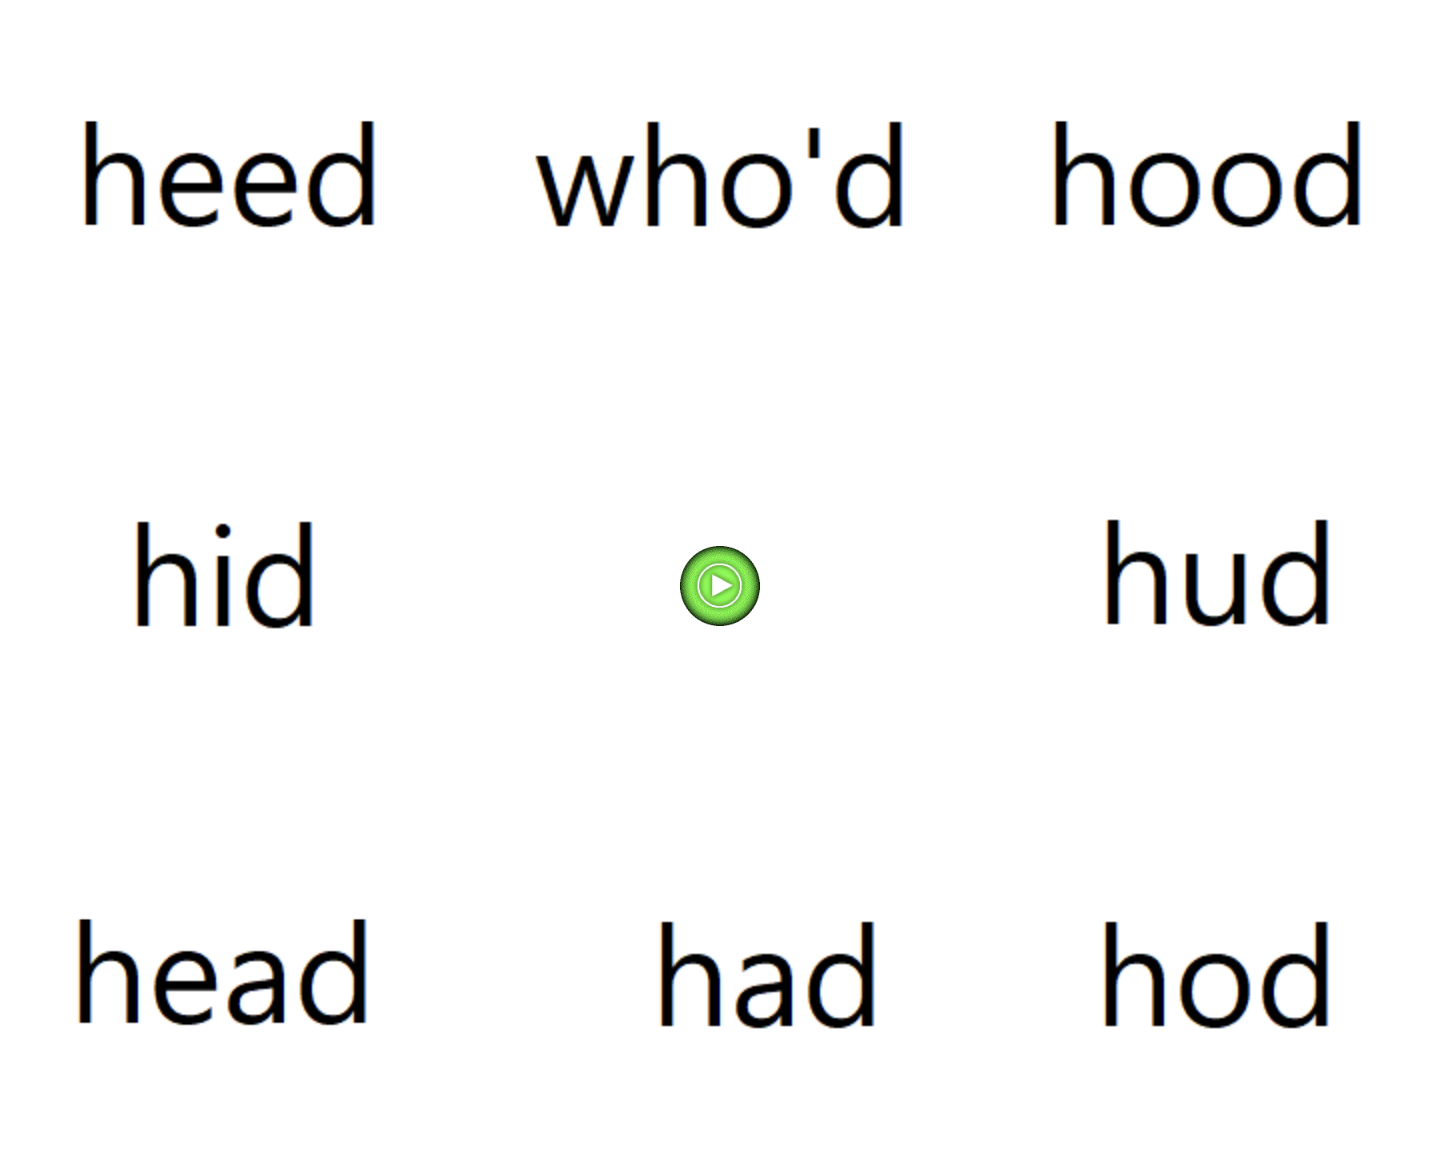
\includegraphics[width=0.4\linewidth]{figures/response-grid} 

}

\caption{Screen shot of the eight-alternative forced-choice (8-AFC) task used in both Experiment 1a and 1b.}\label{fig:exp-procedure}
\end{figure}

Experiment 1a employs recordings of \emph{hVd} word productions from a female talker of US English, these recordings are `natural' in the sense that they were not synthesized or otherwise phonetically manipulated. One consequence of this is that the formant values of these recordings are clustered around the category means, and thus span only a comparatively small part of the phonetic space. This can limit the statistical power to distinguish between competing accounts. Natural recordings furthermore vary not only along the primary cues to vowel quality in US English (F1, F2) but also along potential secondary cues (e.g., F0, F3, and vowel duration) as well as other unknown properties, which can make it difficult to discern whether the performance of a normalization model is due to the normalization itself or other reasons, e.g., because a normalized cue happens to correlate with another cue that listeners are sensitive to but that is not included in the model.

Experiment 1b thus adopts an alternative approach and uses synthesized vowels. Unlike most previous work, which has used isolated vowels as stimuli \citep{barreda-nearey2012, barreda2021, nearey1989, richter2017}, Experiment 1b uses synthesized \emph{hVd} words to facilitate comparison to Experiment 1a. This allowed us to sample larger parts of the F1-F2 space, which has two advantages. First, it allowed us to collect responses over parts of the formant space for which we expect listeners to have more uncertainty, and thus exhibit more variable responses. This can increase the statistical power to distinguish between competing accounts. Second, differences in the predictions of competing normalization accounts will tend to become more pronounced with increasing distance from the category centers. By collecting responses at those locations, we can thus increase the contrast between competing accounts.

The use of synthesized stimuli does, however, also come with potential disadvantages. Synthesized stimuli can suffer in ecological validity, lacking correlations between cues, and across the speech signal (e.g., due to co-articulation) that are characteristic of human speech. This raises questions about the extent to which processing of such stimuli engages the same mechanisms as everyday speech perception. Additionally, it is possible that the use of robotic sounding synthesized speech affects listener engagement. This can lead to an increased rate of attentional lapses, and thus a decrease in the proportion of trials on which listeners' responses are based on the acoustics of the speech stimulus rather than random guessing \citep[compare, e.g.,][]{kleinschmidt2020, tan-jaeger2024}. By comparing normalization accounts against both natural and synthesized stimuli, we investigate the extent to which the accounts that best describe human perception depend on the type of stimuli used in the experiment.

\subsection{Methods}\label{sec:methods}

\subsubsection{Participants}\label{sec:participants}

We recruited 24 (Experiment 1a) and 24 (Experiment 1b) participants from Amazon's Mechanical Turk. Participants were paid \$6/hour prorated by the duration of the experiments (15 minutes). Participants only saw the experiment advertised, and could only participate in it, if (i) they were located within the US, (ii) had an approval rating of 99\% or higher, (iii) met the software requirements (a recent version of the Chrome browser engine), and (iv) had not previously completed any other experiments on vowel perception in our lab. Before the experiment could be accepted, participants had to confirm that they were (i) native speakers of US English (defined as having spent their childhood until the age of 10 speaking English and living in the United States), (ii) in a quiet room without distractions, (ii) wearing over-the-ear headphones. Participants' responses were collected via Javascript developed by the Human Language Processing Lab at the University of Rochester \citep{kleinschmidt2021}.

An optional post-experiment survey recorded participant demographics using NIH prescribed categories, including participant sex (Male: 27, Female: 20), age (mean = 35.5 years; SD = 11.4; 95\% quantiles = 24-63.25 years), race (White: 36, Asian: 3, Black: 6, multiple: 1, declined to report: 1), and ethnicity (Non-Hispanic: 42, Hispanic: 4, declined to report: 1).

\subsubsection{Materials}\label{sec:stimuli}

Experiment 1a employed \emph{hVd} word recordings by one adult female talker from a phonetically annotated database of L1-US English vowel productions \citep{xie-jaeger2020}. Specifically, we used all 9 recordings of each of the eight \emph{hVd}-words---\emph{heed}, \emph{hid}, \emph{head}, \emph{had}, \emph{hut}, \emph{odd}, \emph{who'd}, \emph{hood} \citetext{\citealp[the use of ``hut'' and ``odd'' rather than ``hud'' and ``hod'' follows][]{assmann2008}; \citealp[but see][]{hillenbrand1995}}.

The stimuli for Experiment 1b were synthesized from a single \emph{had} recording used in Experiment 1a. Specifically, we used a script \citep[based on descriptions in][]{wade2007} in Praat \citep{boersma-weenink2022} to concatenate the original /h/ with a synthesized vowel and the original /d/ recording. Unlike in Experiment 1a, all eight words thus had an \emph{hVd} context (including ``hud'' and ``hod'', rather than ``hut'' and ``odd''). The Praat script first segmented the original \emph{had} token into /h/, /ae/ and /d/ portions. It then filtered the /h/ sound inversely with its LPC, and concatenated this neutral fricative sound with a complex waveform generated from the pitch and intensity patterns of the original vowel, to create a neutral hV-section that did not reflect any vocal tract resonances. The script then created a formant grid that filtered the hV-section to create the intended vowel, and finally concatenated this segment to the final /d/ to create an \emph{hVd} word. For each \emph{hVd} word, the formant grid was populated with the F1, F2 and F3 values that we handed to the script at five time-points transitioning from the /h/ to the vowel, to the final /d/ through linear interpolation. Formant bandwidths were 500 Hz at the initial two time-points (the /h/ and beginning of transition to vowel), and then decreased linearly during vowel onset and throughout the final three time-points to 50 Hz (F1), 100 Hz (F2), 200 Hz (F3), 300 Hz (F4), and 400 Hz \citep[F5-F8, following][]{wade2007}. The bandwidth manipulation implied that formants became stronger as the vowel unfolded (see Figure \ref{fig:spectrograms}). We used this approach to create synthesized vowels for arbitrary F1-F2 combinations. F3 was set based on those F1-F2 values. Specifically, we ran a linear regression over the natural productions of the talker from Experiment 1a, predicting F3 from F1, F2 and their interaction. We then used that regression to predict F3 values for any F1-F2 combination in Experiment 1b. F4 to F8, as well as vowel duration, were held identical across all tokens \citep[using the same values as][]{wade2007}.



\begin{figure}

{\centering \subfloat[natural \emph{heed}\label{fig:spectrograms-1}]{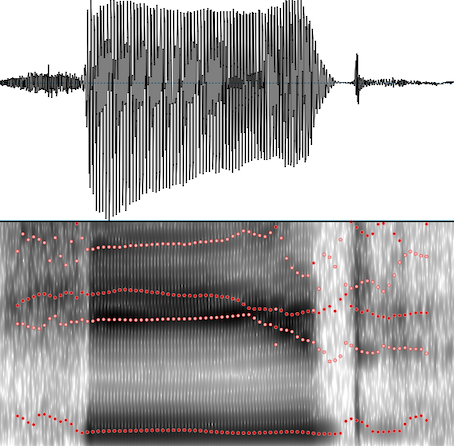
\includegraphics[width=0.2\linewidth]{figures/spectrogram_heed_1a} }\subfloat[natural \emph{hid}\label{fig:spectrograms-2}]{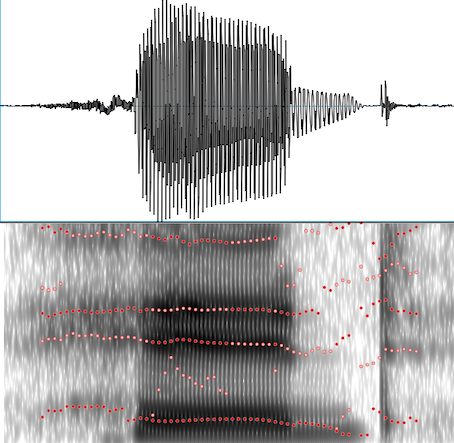
\includegraphics[width=0.2\linewidth]{figures/spectrogram_hid_1a} }\subfloat[natural \emph{odd}\label{fig:spectrograms-3}]{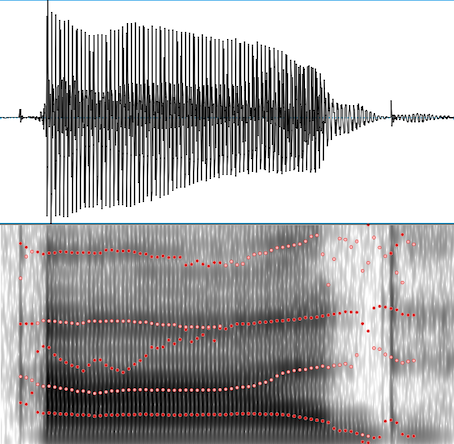
\includegraphics[width=0.2\linewidth]{figures/spectrogram_odd_1a} }\subfloat[natural \emph{hood}\label{fig:spectrograms-4}]{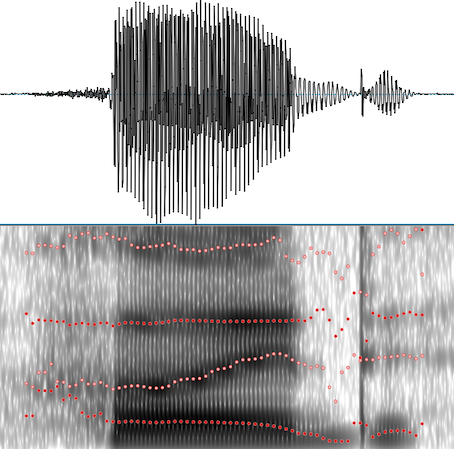
\includegraphics[width=0.2\linewidth]{figures/spectrogram_hood_1a} }\newline\subfloat[resynthesized \emph{heed}\label{fig:spectrograms-5}]{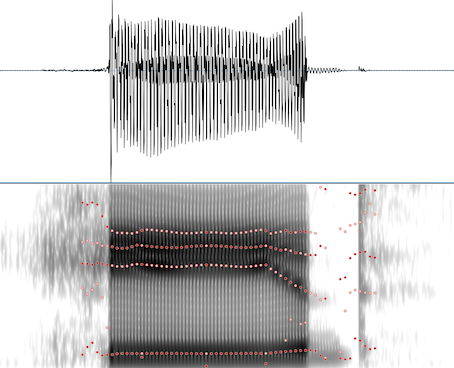
\includegraphics[width=0.2\linewidth]{figures/spectrogram_heed} }\subfloat[resynthesized \emph{hid}\label{fig:spectrograms-6}]{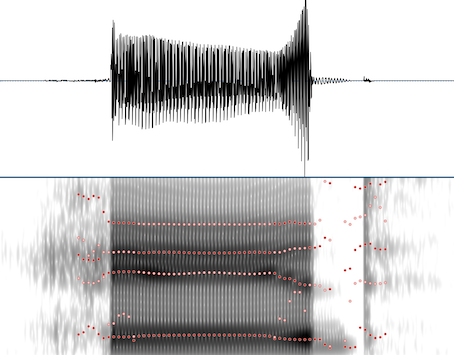
\includegraphics[width=0.2\linewidth]{figures/spectrogram_hid} }\subfloat[resynthesized \emph{hod}\label{fig:spectrograms-7}]{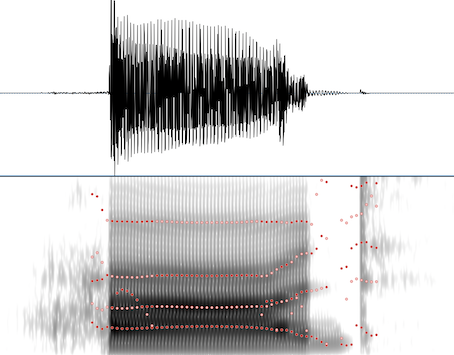
\includegraphics[width=0.2\linewidth]{figures/spectrogram_hod} }\subfloat[resynthesized \emph{hood}\label{fig:spectrograms-8}]{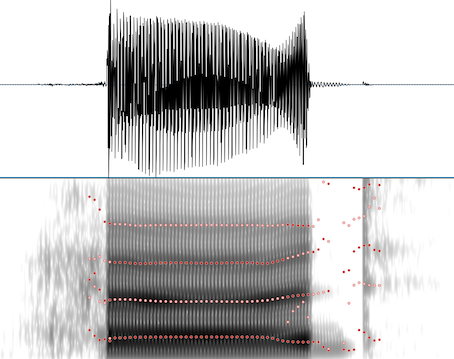
\includegraphics[width=0.2\linewidth]{figures/spectrogram_hood} }\newline

}

\caption{\textbf{Top:} Spectrograms of four natural recordings from Experiment 1a. \textbf{Bottom:} Same for four synthesized tokens with similar formant values from Experiment 1b.}\label{fig:spectrograms}
\end{figure}

We generated 146 synthesized \emph{hVd} recordings that spanned the F1 and F2 space. The specific F1-F2 locations chosen were determined by a mix of modeling (using ideal observers described in the next section to predict listeners' categorization responses) and intuition. Specifically, we selected 64 recordings that we expected to fall within the bivariate 95\% confidence intervals (CIs) of the eight US English monophthongs, and 82 recordings that we expected to fall between those CIs. Figure \ref{fig:human-performance} under \emph{Results} shows the distribution of stimuli for both experiments. Of note, our procedure also generated formant combinations that are physiologically unlikely to have all been produced by the same talker during `normal' vowel production \citep[also known as ``off-template'' instances,][]{nearey1978}.

\subsubsection{Procedure}\label{sec:procedure}

The procedure for both experiments was identical. Live instances of each experiment can be found at \url{https://www.hlp.rochester.edu/experiments/DLPL2S/experiment-A/experiments.html}. At the start of the experiment, participants acknowledged that they met all requirements and provided consent, as per the Research Subjects Review Board of the University of Rochester. Before starting the experiment, participants performed a sound check. Participants were then instructed to listen to a female talker saying words, and click on the word on screen to report what word they heard. On each trial, all eight \emph{hVd}-words were displayed on screen. Half of the participants in each experiment saw the response options organized as in Figure \ref{fig:exp-procedure} (resembling the IPA representation of a vowel space), half saw the response options in the opposite order (flipping top and bottom and left and right in Figure \ref{fig:exp-procedure}). Each trial started with the response grid on screen, together with a light green dot centered on screen. After 1000 ms, an \emph{hVd} recording played, and participants indicated their response by a mouse-click. After a 1000 ms intertrial interval, the screen reset, and the next trial started.

In both experiments, participants heard two blocks of the materials described in the previous sections, for a total of 144 trials in Experiment 1a and 292 trials in Experiment 1b. Presentation within each block was randomized for each participant. Participants were not informed about the block structure of the experiment.

After completing the experiment, participants filled out a language background questionnaire and the optional demographic survey. On average, participants took 10.3 minutes to complete Experiment 1a (SD = 6.6) and 18.4 minutes for Experiment 1b (SD = 7.3).

\subsubsection{Exclusions}\label{exclusions}

We excluded participants who failed to follow instructions and did not wear over-the-ear headphones (as indicated in the post-experiment survey). We also excluded participants with mean (log-transformed) reaction times that were unusually slow or fast (absolute z-score over by-participant means \textgreater{} 3), or if they clearly did not do the task (e.g., by answering randomly). This excluded 6 participants from Experiment 1a and 2 from Experiment 1b (for details, see \ref{sec:SI-exclusions}).

We further excluded all trials that were unusually fast or slow. Specifically, we first z-scored the log-transformed response times \emph{within each participant} and then z-scored these z-scores \emph{within each trial} across participants. Trials with absolute z-scores \textgreater{} 3 were removed from analysis. This double-scaling approach was necessary as participants' response times decreased substantially over the first few trials and then continued to decrease less rapidly throughout the remainder of the experiment. The approach removes response times that are unusually fast or slow \emph{for that participant at that trial}, while avoiding specific assumptions about the shape of the speed up in response times across trials. This excluded 1.2\% of the trials in Experiment 1a and 1.1\% in Experiment 1b. This left for analysis 2565 observations from 18 participants in Experiment 1a, and 6354 observations from 22 participants in Experiment 1b.

\subsection{Results}\label{sec:experiment-results}

Participants' categorization responses in Experiments 1a and 1b are shown in Figure \ref{fig:human-performance}, with larger labels indicating recordings that participants agreed on more.\footnote{\citet{shannon1948} response entropy is defined as \(H(x) = -\sum_{i=1}^{n} P(x_{i}) \log P(x_{i})\). The maximum possible response entropy for an 8-way response choice is 3 bits, which means that all eight vowels are responded equally often. The minimum response entropy = 0 bits, which means that the same vowel is responded all the time.} We make two observations. The first pertains to the degree of (dis)agreement between the two experiments. The second observation pertains to the degree of (dis)agreement across participants within each experiment.

\subsubsection{Similarities and differences between Experiments 1a and 1b}\label{similarities-and-differences-between-experiments-1a-and-1b}

\begin{figure}

{\centering \includegraphics[width=0.9\linewidth]{../../figures/knitted/human-performance} 

}

\caption{Summary of listeners' categorization responses in Experiments 1a and 1b in F1-F2 space. The vowel label indicates the most frequent response provided across participants on each test location. Size indicates how consistent responses were across participants, which larger symbols indicating more consistent responses (lower entropy). F1-F2 combinations below the gray dashed line are articulatory unlikely to come from the same talker.}\label{fig:human-performance}
\end{figure}



Unsurprisingly, participants in both experiments divided the F1-F2 space into the eight vowel categories in ways that qualitatively resembled each other (after taking into account that Experiment 1b covers a larger range of F1-F2 values). Also unsurprisingly, there were some differences between participants' responses across the two experiments, at least when plotted in Hz. For example, {[}\ipatext{u}{]} rarely was the most frequent response in Experiment 1b, even for stimuli that were predominantly categorized as {[}\ipatext{u}{]} in Experiment 1a. There are at least two reasons to expect such differences. First, stimuli with similar F1-F2 values across the two experiments still differed in other acoustic properties (e.g.~vowel duration or F3). These acoustic differences might have affected participants' responses. Second, it is possible that \emph{formant normalization} affected participants' responses---i.e., the very mechanism we seek to investigate in the remainder of the paper. The two experiments differ in the means, variances, and other statistical properties that some normalization accounts predict to affect perception. As a consequence, Hz might not be the space in which we should expect identical responses across experiments.

Similarly, the two experiments differed in the extent to which participants agreed with each other. Participants in Experiment 1b exhibited overall less agreement in their responses (mean by-item response entropy = 0.45 bits, SE = 0.01) than participants in Experiment 1a (mean by-item response entropy = 0.23 bits, SE = 0.02). This was expected given that Experiment 1b explored the entire F1-F2 space, including---by design---formant combinations located \emph{between} the centers of the natural vowel categories. Experiment 1b therefore achieved its goal of eliciting less categorical response distributions, which is expected to facilitate comparison of competing normalization accounts.\footnote{Note that participants in Experiment 1a exhibited high agreement on {[}\ipatext{ʌ}{]}, {[}\ipatext{æ}{]}, and {[}\ipatext{ɑ}{]}, despite the close proximity between, and partial overlap of, these vowels in F1-F2 space. To understand this pattern, it is important to keep in mind that the recordings for {[}\ipatext{ʌ}{]} and {[}\ipatext{ɑ}{]} differed from the recordings for other stimuli in their word onset (``odd'' for {[}\ipatext{ɑ}{]}) or offset (``hut'' for {[}\ipatext{ʌ}{]}).}

Auxiliary analyses presented in the SI (\ref{sec:SI-aux-entropy}) suggest that \emph{some but not all} of the differences in response entropy between the two experiments were caused by the placement of the stimuli in formant space: when comparing categorization responses for tokens from the two experiments with similar acoustic properties (differences of \(\le 30\) Hz along F1 and F2), response entropies still differed substantially (for N = 40 acoustically similar tokens, mean by-item response entropy for Experiment 1a = 0.18 bits, SE = 0.03; Experiment 1b = 0.39 bits, SE = 0.03). We see two mutually compatible explanations. First, similar to the differences between experiments in the dominant response pattern discussed above, differences in the degree of agreement between participants might originate in \emph{normalization}. Second, it is possible that the relation between formants in the synthesized stimuli or some other unknown acoustic-phonetic differences between the experiments explain the difference in response. For example, the absence of vowel inherent spectral change (VISC) or differences in tilt in the synthesized stimuli might have deprived listeners of information that is actually crucial for establishing phonemic identity \citep{hillenbrand-nearey1999}. This would result in increased uncertainty on each trial, leading to increased entropy of listeners' responses. The computational study we present below shed some light on these two mutually compatible possibilities.

\subsubsection{Similarities and differences between participants}\label{similarities-and-differences-between-participants}

Since the intended category was known for Experiment 1a, it was possible to calculate participants' recognition accuracy. As also evident in the left panel of Figure \ref{fig:human-performance}, participants' most frequent response \emph{always} matched the intended vowel in Experiment 1a. Overall, participants' responses matched the intended vowel on 81.2\% (SE = 4.8\%) of all trials (Experiment 1b had no such ground truth). This is much higher than chance (12.5\%). It is, however, also quite a bit lower than 100\%. To better understand the reasons for this, Figure \ref{fig:human-confusion}A plots the confusion matrix. This suggests that participants' performance was largely affected by confusions between {[}\ipatext{ɪ}{]}-to-{[}\ipatext{ɛ}{]} (\emph{hid}-to-\emph{head}), {[}\ipatext{ɛ}{]}-to-{[}\ipatext{æ}{]} (\emph{head}-to-\emph{had}), and {[}\ipatext{u}{]}-to-{[}\ipatext{ʊ}{]} (\emph{who'd}-to-\emph{hood}).



\begin{figure}[!ht]

{\centering \includegraphics[width=0.9\linewidth]{../../figures/knitted/human-confusion} 

}

\caption{Category confusability in Experiments 1a and 1b. \textbf{Panel A} summarizes the category confusability. Since correct responses were not defined for Experiment 1b, we grouped items along the x-axis based on most frequent response that listeners provided (for Experiment 1a, this was always identical to the intended response). Response percentages sum to 100 in each column, showing the response distribution depending on the most frequent response. \textbf{Panel B} summarizes individual differences across listeners, in terms of the listener-specific confusability of {[}\ipatext{ɪ}{]} with {[}\ipatext{ɛ}{]} (x-axis), {[}\ipatext{ɛ}{]} with {[}\ipatext{æ}{]} (y-axis), and {[}\ipatext{u}{]} with {[}\ipatext{ʊ}{]} (color fill).}\label{fig:human-confusion}
\end{figure}

One plausible explanation for this pattern of vowel confusions lies in the substantial variation that exists across US English dialects \citep{atlasnae}. Differences in the realization of vowel categories, and associated representations, across dialects will directly affect the expected classification for any given token. In addition, listeners might differ in terms of experience with different dialects, or in the dialect they attribute to the talker who produced the stimuli. To test this hypothesis, we calculated the {[}\ipatext{ɪ}{]}-to-{[}\ipatext{ɛ}{]}, {[}\ipatext{ɛ}{]}-to-{[}\ipatext{æ}{]}, and {[}\ipatext{u}{]}-to-{[}\ipatext{ʊ}{]} confusion rates for each participant in Experiment 1a. These data are summarized in the left panel of Figure \ref{fig:human-confusion}B. The data in the left panel suggest that most participants in Experiment 1a either heard {[}\ipatext{ɪ}{]} tokens consistently as the intended {[}\ipatext{ɪ}{]} (clustering on the left side of the panel) or as {[}\ipatext{ɛ}{]} (clustering on the right side of the panel). Only a few participants exhibited mixed responses for items intended to be {[}\ipatext{ɪ}{]}. Tellingly, many of the participants who exhibited increased {[}\ipatext{ɪ}{]}-to-{[}\ipatext{ɛ}{]} confusion \emph{also} exhibited increased {[}\ipatext{ɛ}{]}-to-{[}\ipatext{æ}{]} confusion. This is precisely what would be expected by listeners who assume a dialect in which these vowels are articulated lower (with higher F1) than in the dialect of the talker in Experiment 1a. A similar, but less pronounced, pattern was also found with regard to {[}\ipatext{u}{]}-to-{[}\ipatext{ʊ}{]} confusions.\footnote{{[}\ipatext{u}{]} has been undergoing changes in many varieties of US English. Whereas the talker in Experiment 1a produces {[}\ipatext{u}{]} with low F1 and F2 (high and back), other L1 talkers of US English produce this vowel considerably more forward (higher F2).} Finally, a qualitatively similar relation between {[}\ipatext{ɪ}{]}-to-{[}\ipatext{ɛ}{]}, {[}\ipatext{ɛ}{]}-to-{[}\ipatext{æ}{]}, and {[}\ipatext{u}{]}-to-{[}\ipatext{ʊ}{]} confusions was also observed in Experiment 1b (right panel of Figure \ref{fig:human-confusion}B), though the pattern was unsurprisingly less pronounced given that the stimuli in Experiment 1b by design often fell into the ambiguous region \emph{between} vowels. Taken together, Experiments 1a and 1b thus suggest that systematic dialectal differences between participants may be a substantial contributor of the relatively low correct classification rate observed for Experiment 1a.

This highlights two important points. First, the data from Experiment 1a demonstrate the perceptual challenges associated with an unfamiliar talker: in the absence of lexical or other context to distinguish between the eight available response options, listeners can only rely on the acoustic information in the input. In such a scenario, even listeners who are in principle familiar with the dialect spoken by the talker have comparatively little information to determine the talker's dialect, making apparent what Matt \citet{winn2018} aptly summarizes as ``speech {[}perception{]} is not as acoustic as {[}we{]} think''. Second, when dialect variability is taken into account, listeners' recognition accuracy improved substantially. After removing 7 listeners who heard more than 50\% of the {[}\ipatext{ɪ}{]} items as {[}\ipatext{ɛ}{]}, \emph{all} vowels were correctly recognized at least 88.3\% of the time (overall accuracy = 95.9\%). This suggests that dialect differences affected the recognition of all vowels. This aspect of our results serves as an important reminder that formant normalization is only expected to erase inter-talker variability associated with \emph{physiological} differences: variation in dialect, sociolect, or other non-physiologically-conditioned variation pose separate challenges to human perception, and require additional mechanisms \citep[see discussion in][]{barreda2021, weatherholtz-jaeger2016}. This introduces noise---variability in listeners' responses that cannot be accounted for by normalization---to any comparison of normalization accounts, potentially reducing the power to detect differences between accounts.

\section{Comparison of normalization accounts}\label{comparison-of-normalization-accounts}

In order to evaluate normalization accounts against speech perception, it is necessary to map the phonetic properties of stimuli---under different hypotheses about normalization---onto listeners' responses in Experiments 1a and 1b. Previous work has done so by directly predicting listeners' responses from the raw or normalized phonetic properties of stimuli \citep{apfelbaum-mcmurray2015, barreda2021, crinnion2020, mcmurray-jongman2011, nearey1989}. For example, McMurray and Jongman used multinomial logistic regression to predict 8-way fricative categorization responses in US English \citep[see also][]{barreda2021}.

Here we pursued an alternative approach by committing to a core assumption common to contemporary theories of speech perception: that listeners acquire implicit knowledge about the probabilistic mapping from acoustic inputs to linguistic categories, and draw on this knowledge during speech recognition \citetext{\citealp[e.g., TRACE,][]{mcclelland-elman1986}; \citealp[exemplar theory,][]{johnson1997}; \citealp[Bayesian accounts,][]{luce-pisoni1998}; \citealp{nearey1990}; \citealp{norris-mcqueen2008}; \citealp[ASR-inspired models like DIANA or EARSHOT,][]{bosch2015}; \citealp{magnuson2020}}. Using a general computational framework for adaptive speech perception \citep[ASP,][]{xie2023} we trained Bayesian ideal observers to capture the expectations that a `typical' L1 adult listener might have about the formant-to-vowel mappings of US English. We approximated these expectations using a database of L1-US English vowel productions \citep{xie-jaeger2020}---transformed to reflect the different normalization accounts. We then ask which of the different ideal observer models---corresponding to different hypotheses about formant normalization---best predicts listeners' responses in Experiments 1a and 1b.

A welcome side effect of this is that far fewer degrees of freedom (DFs) are required to predict listeners' responses. For example, using ordinary multinomial logistic regression trained on our perceptual data to predict 8-way vowel categorization as a function of F1, F2 and their interaction would require up to 28 DFs. This problem increases with the number of cues considered. Because the model is trained on data that is independent of our perceptual data, the ASP-based approach we employ instead uses only 2 DFs (i.e., parameters estimated based on our perceptual data) to mediate the mapping from stimuli properties to listeners' responses, regardless of the number of cues considered. Over the next few sections, we describe how this parsimony is made possible through a commitment to strong linking hypotheses motivated by theories of speech perception.

\subsection{Methods}\label{methods}

\subsubsection{\texorpdfstring{A general-purpose categorization model for \(J\)-AFC categorization tasks}{A general-purpose categorization model for J-AFC categorization tasks}}\label{sec:predict-perception}

\begin{figure}[!ht]
\begin{center}
   \tikz{ %
    \node[obs] (r) {$r$} ; %
    \node[const, right=of r, xshift=-.009cm] (r_description) {{\em categorization response}} ; %
    \node[det, below=of r] (decision) {} ; %
% decisions
    \node[const, right=of decision, xshift=-.009cm] (decision_rule) {{\em decision rule} (Luce choice rule)} ; %
    \factor[below=of decision, xshift=-.009cm, yshift=-.5cm] {response-dist} {left: $\mathcal{M}$} {} {}; %
    \factor[right=of response-dist, xshift=.8cm, yshift=-1cm] {prior-dist} {left: Multi} {} {}; %
    \factor[below=of response-dist, xshift=-.009cm, yshift=-1cm] {multi} {left: Multi} {} {}; %
    \node[latent, right=of response-dist, xshift=1.5cm] (l) {$\lambda$} ; %
    \node[const, right=of l, xshift=-.009cm] (lapse) {{\em lapse rate} ($1$ DF)} ; %
    \node[latent, right=of prior-dist, xshift=.2cm, yshift=-.009cm] (pi_n) {$\pi_{c}$} ; %
    \node[right=of pi_n] (beta_description) {{\em response biases}} ;
% edges
    \edge {decision} {r} ;
    \edge {response-dist} {decision} ; %
    \edge {multi} {response-dist} ; %
    \edge {prior-dist} {response-dist} ; %
    \edge {prior-dist} {multi} ; %
    \edge {l} {response-dist} ; %
    \edge {pi_n} {prior-dist} ;
% representations
    \factor[below=of multi,  yshift=-1cm] {x_prime} {left:$\mathcal{N}$} {} {}; %
     %\node[above=of x_prime] (dots) {$\vdots$} ; %
    \node[obs, right=of x_prime, yshift=.5cm, xshift=.3cm] (mu_n) {$\mu_{c}$} ; %
    \node[obs, right=of x_prime, yshift=-.5cm, xshift=.3cm] (sigma_n) {$\Sigma_{c}$} ; %
    \node[right=of mu_n] (mu_n_description) {{\em category means} (estimated from phonetic database)} ;
    \node[right=of sigma_n] (sigma_n_description) {{\em category covariance} (estimated from phonetic database)} ;

% edges
    \edge {x_prime} {multi} ; %
    \edge {mu_n} {x_prime} ; %
    \edge {sigma_n} {x_prime} ; %
% noise
    \node[det, below=of x_prime, yshift=-1cm] (x_prime2) {} ; %
      %\node[above=of x_prime2] (dots) {$\vdots$} ; %
    \node[latent, right=of x_prime2] (sigma_noise) {$\Sigma_{noise}$} ; %
    \node[right=of sigma_noise, xshift=-.3cm] (sigma_noise_description) {{\em internal \& external noise} (1 DF)} ;
%edges
    \edge {x_prime2} {x_prime} ; %
    \edge {sigma_noise} {x_prime2} ; %
% normalization
    \node[det, below=of x_prime2, yshift=-.4cm] (x_prime3) {} ; %
    \node[obs, right=of x_prime3] (theta) {$\theta$} ; %
    \node[right=of theta] (theta_description) {{\em normalization parameters} (estimated from phonetic database \& stimuli)} ; %
    \node[obs, below=of x_prime3] (x) {x} ; %
    \node[const, right=of x, xshift=-.009cm] (x_description) {{\em phonetic properties of stimulus} (formants)} ;
%edges
    \edge {x_prime3} {x_prime2} ; %
    \edge {theta} {x_prime3} ; %
    \edge {x} {x_prime3} ; %
}

\caption{Graphical model of ASP's general categorization framework (adapted for the current purpose from Xie et al., 2023, Figure 4). Here $J=8$ (the eight vowel response options in Experiments 1a and 1b). We use this framework to compare normalization accounts against listeners' categorization responses from Experiments 1a and 1b. Filled gray circles represent variables that are known to the researcher. Empty circles represent latent variables that are not observable. Diamonds represent variable-free processes, annotated with the distributions resulting at that level of the model: $\mathcal{N}$(ormal), Multi(nomial), and $\mathcal{M}$(ixture) distributions.} \label{fig:model-perceptual-decision-making}
\end{center}
\end{figure}

Figure \ref{fig:model-perceptual-decision-making} summarises ASP's categorization model for a \(J\)-alternative forced-choice task \citep[for an in-depth description, we refer to][]{xie2023}. The model combines Bayesian ideal observers \citetext{\citealp[as used in e.g.,][]{clayards2008}; \citealp{feldman2009}; \citealp{norris-mcqueen2008}; \citealp{xie2021}; \citealp[for a closely related approach, see also][]{nearey-hogan1986}} with psychometric lapsing models \citep{wichmann-hill2001}. To reduce researchers' degrees of freedom, we adopt all assumptions made in \citet{xie2023}, and do not introduce additional assumptions.

Starting at the bottom of the figure, the phonetic input \(x\) is normalized. Here, \(x\) = the F1 and F2 of our stimuli (the SI, \ref{sec:SI-F1F3} reports additional analyses that instead employ F1-F3; these analyses support the same conclusion presented here, and we mention them below where relevant). The specific computations applied to the input \(x\) depend on the normalization accounts (see Table \ref{tab:norm-accounts}). We use \(\theta\) to refer to the parameters required by the normalization account. For example, for the uniform scaling account \citep{nearey1978}, \(\theta\) is the overall mean of all log-transformed formants. For Lobanov normalization \citep{lobanov1971}, \(\theta\) is a vector of means and standard deviations for each formant (in Hz).

The normalized input is then perturbed by perceptual and environmental noise. Following \citet{feldman2009}, this noise is assumed to be Gaussian distributed centered around the transformed stimulus with noise variances that are independent and identical for all formants (i.e., \(\Sigma_{noise}\) is a diagonal matrix, and all diagonal entries have the same value). Next, the likelihood of the normalized percept under each of the eight vowel categories is calculated, \(p(F1, F2 | vowel)\). This requires specifying listeners' expectations about the cue-to-category mapping (listeners' likelihood function). We followed \citet{xie2023} and previous work and assume that each vowel maps onto a multivariate Gaussian distribution over the phonetic cues, here bivariate Gaussians over F1 and F2 \citep[cf.][]{clayards2008, feldman2009, kleinschmidt-jaeger2015, norris-mcqueen2008, xie2021}. The posterior probability of each vowel is obtained by combining its likelihood with its prior probability or response bias \(\pi_c\), according to Bayes theorem:\footnote{For Gaussian noise and Gaussian category likelihoods, the resulting noise-convolved likelihood is a Gaussian with variance equal to the sum of the noise and category variances \citep{kronrod2016}.}

\begin{equation}
 p(vowel = c |F1, F2) = \frac{\mathcal{N}(F1, F2| \mu_c, \Sigma_c + \Sigma_{noise}) \times \pi_c}{\sum_{c_i} \mathcal{N}(F1, F2|\mu_{c_i}, \Sigma_{c_i} + \Sigma_{noise}) \times \pi_{c_i}} \label{eq:Bayes-rule-normal}
\end{equation}

Up to this point, the model is identical to a standard Bayesian ideal observer over noisy input \citep{feldman2009, kronrod2016} for which the input has been transformed based on the normalization account. ASP's categorization model adds to this the potential that participants experience attentional lapses---or for other reasons do not respond based on the input---on some proportion of all trials \citep[\(\lambda\), as in standard psychometric lapsing models,][]{wichmann-hill2001}. On those trials, the posterior probability of a category is determined solely by participants' response bias, which we assume to be identical to the response bias on non-lapsing trials \citep[following][]{xie2023}. This results in a posterior that is described by weighted mixture of two components, describing participants' posterior on non-lapsing and lapsing trials, respectively:

\begin{equation}
 p(vowel = v|F1, F2) = (1-\lambda) \frac{\mathcal{N}(F1, F2| \mu_c, \Sigma_c + \Sigma_{noise}) \times \pi_c}{\sum_{c_i} \mathcal{N}(F1, F2|\mu_{c_i}, \Sigma_{c_i} + \Sigma_{noise}) \times \pi_{c_i}} + \lambda \frac{\pi_c}{\pi_{c_i}} \label{eq:Bayes-rule-ASP}
\end{equation}

Finally, a decision rule is applied to the posterior to determine the response of the model, conditional on the input (one of the eight vowels in Experiments 1a and 1b). We followed the gross of research on speech perception and assume Luce's choice rule \citetext{\citealp{luce1959}; \citealp[for discussion, see][]{massaro-friedman1990}}. Under this choice rule, the model can be seen as sampling from the posterior, responding with each category proportional to that category's posterior probability.

Next, we describe how we estimated the \(\theta\)s, \(\mu_c\)s and \(\Sigma_c\)s for each normalization account from a phonetic database. We use this database as a---very coarse-grained---approximation of a the speech input a `typical' listener might have experienced previously. By fixing \(\theta\), \(\mu_c\) and \(\Sigma_c\) based on the distribution of phonetic cues in the database, we substantially reduce the DFs that are allowed to mediate the mapping from stimulus properties to listeners' responses \citep[following][]{xie2023}. In addition, this approach naturally penalizes overly complex models by validating these against out-of-sample data. Finally, we describe how we fit the remaining parameters as DFs to participants' responses from Experiments 1a and 1b.

\subsubsection{\texorpdfstring{Modeling listeners' prior experience (and guarding against overfitting): \(\theta\), \(\mu_c\), and \(\Sigma_c\)}{Modeling listeners' prior experience (and guarding against overfitting): \textbackslash theta, \textbackslash mu\_c, and \textbackslash Sigma\_c}}\label{modeling-listeners-prior-experience-and-guarding-against-overfitting-theta-mu_c-and-sigma_c}

By fixing \(\theta\), \(\mu_c\), and \(\Sigma_c\) based on a database of vowel \emph{productions}, we impose strong constraints on the functional flexibility of the model in predicting listeners' responses. This benefit is made possible by committing to a strong linking hypothesis---that listeners' categories are learned from, and reflect, the distributional mapping from formants to vowels in previously experienced speech input \citep[e.g.,][]{abramson-lisker1973, massaro-friedman1990, nearey-hogan1986}. The database we use to approximate listeners' prior experience was originally developed to compare the production of L1 and L2 speakers \citep{xie-jaeger2020}. It contains 9-10 recordings of the 8 \emph{hVd} words from each of 17 (5 female) L1 talkers of a Northeastern dialect of US English (ages 18 to 35 years old). Since Experiments 1a and 1b used recordings of one of these talkers, we excluded that talker prior to fitting training ideal observers on the data. In total, this yields 5842 recordings that are annotated for F0, F1-F3, and vowel duration. The SI (\ref{sec:SI-xie-jaeger}) summarizes the distribution of these cues, and how the different normalization accounts affect those distributions.

To avoid over-fitting the ASP model to the database, we used 5-fold cross-validation: we randomly split the \citet{xie-jaeger2020} database into five approximately evenly-sized folds \citep[following][]{persson-jaeger2023}. This split was performed within each vowel to guarantee that all five folds had the same relative amount of data for each vowel category. These splits were combined into five training sets, each containing one of the folds (20\% of the data). This way, each training set was different from the others, increasing the variability between sets.\footnote{We intentionally did \emph{not} split the data within talkers since normalization accounts are meant to make speech perception robust to cross-talker variability. Further, splitting the data by speaker rather than by vowel category avoids the potential for biases in the normalization parameter estimates for different speakers in the case of missing or unbalanced tokens across vowel categories, see \citep{barreda-nearey2018}. Additional analyses not reported here confirmed that the same results are obtained when splits are performed within talkers and within vowels (except that this lead to smaller CIs, and thus \emph{more} significant differences, in Figure \ref{fig:plot-io-optimal}). These analyses can be replicated by downloading the R markdown document this article is based on from our OSF (see comments in our code).}

For each training set and for each normalization account, we then estimated the required normalization parameters \(\theta\) for all talkers, and normalized all formants based on those talker-specific parameters.This yielded 5 (training sets) * 20 (accounts) = 100 normalized training sets. For each of these normalized training sets, we fit the category means, \(\mu_c\), and covariance matrices, \(\Sigma_c\), of all eight vowels, using the \texttt{R} package \texttt{MVBeliefUpdatr} \citep{R-MVBeliefUpdatr}.\footnote{Alternatively, it would be possible to treat these parameters as DFs in the link to listeners' responses, and infer them from the responses in Experiments 1a and 1b \citep[cf.,][]{kleinschmidt-jaeger2016}. This approach would afford the model with a high degree of functional flexibility, regardless of which normalization approach is applied (similar to previous approaches that have employed, e.g., multinomial logistic regression).}

This yielded 100 ideal observer models, 5 for each of the 20 normalization accounts in Table \ref{tab:norm-accounts}. Of note, the 20 ideal observers fit on each fold differ \emph{only} in the assumptions they make about the normalization that is applied to cues before they are mapped onto the eight vowel categories. Figure \ref{fig:io-plot-categories} visualizes the resulting bivariate Gaussian categories for four of the 20 normalization accounts. This illustrates one advantage of the cross-validation approach: it takes a modest step towards simulating differences across listeners' prior experience (represented by the five different folds).



\begin{figure}[!ht]

{\centering \includegraphics[width=0.95\linewidth]{../../figures/knitted/io-plot-categories} 

}

\caption{Visualizing the bivariate Gaussian categories (prior to adding \(\Sigma_{noise}\)) of four example normalization accounts in F1-F2 space. Separate ellipses are shown for each of the five training sets (each set corresponds to one set of eight ellipses). The relative stability of the category ellipses across training sets indicates that the database is sufficiently large for the present purpose.}\label{fig:io-plot-categories}
\end{figure}

\subsubsection{Transforming the stimuli from Experiments 1a and 1b into the normalized phonetic spaces}\label{transforming-the-stimuli-from-experiments-1a-and-1b-into-the-normalized-phonetic-spaces}

Next, we transformed the stimuli of Experiments 1a and 1b into the formant space defined by the 20 normalization accounts in Table \ref{tab:norm-accounts}. This requires estimating the required normalization parameters \(\theta\) for each experiment and normalization account. We calculated these \(\theta\)s over all stimuli (of each experiment and normalization account). For example, for the uniform scaling account \citep{nearey1978}, we calculated the overall mean of all log-transformed formants over all stimuli. For Lobanov normalization \citep{lobanov1971}, we calculated the mean and standard deviation of each formant (in Hz) over all stimuli. For each combination of experiment and normalization account, we then normalized the stimuli using those parameter estimates.

Combining the 100 normalized training sets described in the previous section with the matching normalized stimuli from each of the two experiments yielded 200 data sets.

\subsubsection{\texorpdfstring{Noise (\(\Sigma_{noise}\)) and attentional lapses (\(\lambda\))}{Noise (\textbackslash Sigma\_\{noise\}) and attentional lapses (\textbackslash lambda)}}\label{noise-sigma_noise-and-attentional-lapses-lambda}

Finally, we describe the two parameters of the ASP model that we fit against listeners' responses in Experiments 1a and 1b. These two parameters constitute the only DFs that mediate the link from ideal observers' predictions to listeners' responses, and which are specifically tuned to these. The first DF (\(\Sigma_{noise}\)) models the effects of internal (perceptual) and external (environmental) noise on listeners' perception. While previous work provides estimates of the internal noise in formant perception, these estimates were obtained under \emph{assumptions} about the relevant formant space. For example, \citet{feldman2009} estimated the internal noise variance to be about 15\% of the average category variance along F1 and F2. This estimate was based on the assumption that human speech perception transforms vowel formants into Mel, without further normalization. Since we aim to \emph{test} which normalization account best explains speech perception, we cannot rely on this or other internal noise estimates obtained under a single specific assumption. Additionally, internal noise can vary across individuals and external noise can vary across environments (a point particularly noteworthy, given that we conducted Experiments 1a and 1b over the web). We thus allowed the noise variance \(\Sigma_{noise}\) to vary in fitting participants' responses. Following \citet{feldman2009}, we assumed that perceptual noise had identical effects on all formants in the phonetic space defined by the normalization account \citep[see also][]{kronrod2016}. This reduces \(\Sigma_{noise}\) to a single DF, regardless of the normalization account (for details, see SI \ref{sec:SI-optim-process}).

The magnitude of \(\Sigma_{noise}\) affects the slope of the categorization functions that predict listeners' responses from stimulus properties (here, F1 and F2): higher \(\Sigma_{noise}\) imply more shallow categorization slopes. To facilitate comparison of \(\Sigma_{noise}\) values across normalization accounts, we report results in terms of the best-fitting \emph{noise ratios} (\(\tau^{-1}\)), rather than \(\Sigma_{noise}\)s. Specifically, \(\Sigma_{noise}\) is best understood \emph{relative} to the inherent variability of the vowel categories (\(\Sigma_c\)). This variability in turn depends on the phonetic space defined by the normalization account. We thus divide \(\Sigma_{noise}\) by the mean of the diagonals of all \(\Sigma_c\)s to obtain the \emph{noise ratio} \(\tau^{-1}\). For example, noise ratio of 0 corresponds to the absence of any noise, and a noise ratio of 1 corresponds to noise variance of the same magnitude as the average category variance along F1 and F2 in the phonetic space defined by the normalization account.\footnote{This ratio is a generalization of the inverse of the ``meaningful-to-noise variance ratio (\(\tau\))'' used in \citet{kronrod2016}. However, whereas Kronrod and colleagues committed to the simplifying assumption that all categories have identical variance (along all formants), we allowed category variances to differ between vowels, and between F1 and F2 (matching the empirically facts). We merely assume that the \emph{noise} variance is identical across all formants (in the phonetic space defined by the normalization account, e.g., log-Hz for uniform scaling and Hz for Lobanov).} Figure \ref{fig:prediction-landscapes}B illustrates the effects of this noise ratio for Nearey's uniform scaling account.



\begin{figure}[!ht]

{\centering \includegraphics[width=0.95\linewidth]{../../figures/knitted/prediction-landscapes} 

}

\caption{Illustrating the consequences of perceptual and external noise (\(\Sigma_{noise}\)) and attentional lapse rates (\(\lambda\)) on the predicted posterior distribution of vowel categorizations. Shown are the average predicted posteriors across all five folds for Nearey's uniform scaling account. \textbf{Panel A}: Predicted posterior distribution for noise ratio \(\tau^{-1} = \lambda\) = 0. \textbf{Panel B}: Same for \(\tau^{-1}\) = 1 and \(\lambda\) = 0. \textbf{Panel C}: Same for \(\tau^{-1} = 0\) and \(\lambda\) = 0.5. Transparency of a color is determined by that vowel's posterior probability. Contours indicate the highest posterior probability of any vowel (at .4, .5, .7, .95 probability level).}\label{fig:prediction-landscapes}
\end{figure}

Second, participants can attentionally lapse or for other reasons reply without considering the speech input. We thus allowed lapse rates (\(\lambda\)) to vary while fitting human responses. This introduces a second DF, which we fit against listeners' responses. Together, the inclusion of freely varying lapse rates and a uniform response bias allows the ASP models to capture that some unknown proportion of listeners' responses might be more or less random, rather than reflecting properties of the vowel stimuli. This is illustrated in Figure \ref{fig:prediction-landscapes}C.

Finally, participants can have response biases that reflect their beliefs about the prior probability of each category. However, to reduce the DFs fit to participants' responses, we did \emph{not} fit this response bias against listeners' responses (thus avoiding \(J - 1 = 7\) additional DFs). Instead, we assumed uniform response biases---i.e., that listeners believed all eight response options in the experiments to be equally likely (\(\forall c\ \pi_c = .125\)). This decision implies that our models would not be able to capture any potential non-uniformity in listeners' response biases---including potential effects of additional acoustic differences (the absence of {[}h{]} in \emph{odd} or the coda {[}t{]}, rather than {[}d{]} in \emph{hut}) and orthographically particular response options in Experiment 1a (``who'd'', ``odd'', and ``hut''). We do, however, see no reasons to expect this decision to bias the comparison of normalization accounts.

\subsubsection{Fitting normalization accounts to listeners' responses}\label{fitting-normalization-accounts-to-listeners-responses}

For each of the 200 combinations of experiment, normalization account, training set, we used constrained quasi-Newton optimization \citep[as implemented in \texttt{R}'s \texttt{optim()} function]{byrd1995} to find the \(\lambda\) and \(\tau^{-1}\) values that best described listener's responses. Specifically, we used the 100 ideal observers described in the previous sections, applied them to the normalized stimuli of the experiment, and determined which \(\lambda\) and \(\tau^{-1}\) maximized the likelihood of listener's responses (for details, see SI \ref{sec:SI-optim-process}). This procedure yielded five maximum likelihood estimates for both \(\lambda\) and \(\tau^{-1}\) for each combination of experiment and normalization account---one for each training set. All result presented below were validated and confirmed by grid searches over the parameter spaces (SI, \ref{sec:SI-study1-grid-search}).

We compare normalization accounts in terms of the likelihood of listeners' responses under these maximum likelihood estimates of \(\lambda\) and \(\tau^{-1}\). Comparing accounts in terms of their data likelihood, rather than the accuracy of predicting intended productions \citep[e.g.,][]{johnson2020, persson-jaeger2023}, or correlations with human response proportions \citep[e.g.,][]{nearey-assmann1986, hillenbrand-nearey1999}, follows more recent work \citep[e.g.,][]{barreda2021, mcmurray-jongman2011, richter2017, xie2023} and parallels standard approaches to model comparison in contemporary data analysis. We note that this approach puts normalization accounts to a stronger test. For example, a model can exhibit high correlations with listeners' responses even when its predictions are systematically `off'. Similarly, a model can achieve high accuracy in predicting listeners' responses simply because it always predicts the most frequent response, and that response accounts for sufficiently much of the data. In contrast, the likelihood of listeners' responses under a model is a direct measure of how well the model captures the distribution of listeners' responses conditional on the stimulus properties. In particular, data likelihood will be maximized if, and only if, the model-predicted posterior probabilities of each vowel for each stimulus are identical to the proportion with which those vowels occur in listeners' responses.

\subsection{Results}\label{results}

We begin by comparing the fit of different accounts against listeners' responses in Experiments 1a and 1b. Given the comparatively large number of accounts compared here, we provide initial conclusions based on the best-fitting accounts along with the description of the results (more in-depth discussion is provided in the general discussion). Following this comparison, we visualize how different normalization accounts predict the formant space to be divided into the eight vowel categories.

\subsubsection{Comparing normalization accounts in terms of fit against human behavior}\label{comparing-normalization-accounts-in-terms-of-fit-against-human-behavior}



\begin{figure}[!ht]

{\centering \includegraphics[width=0.95\linewidth]{../../figures/knitted/plot-io-optimal} 

}

\caption{Comparison of normalization accounts against listeners' responses. Pointranges indicate mean and 95\% bootstrapped CIs of the log-likelihood summarized over the five training sets (higher is better). Accounts that fit listeners' responses to an extent that is statistically indistinguishable from the best-fitting account are marked by (*). Note that y-axis range differs across panels, and that it is \emph{not} meaningful to compare the absolute log-likelihood values across the two experiments (just as it is not meaningful to compare the data likelihood of regressions that are fit on two different data sets).}\label{fig:plot-io-optimal}
\end{figure}

Figure \ref{fig:plot-io-optimal} compares how well the different normalization accounts fit listeners' responses in Experiments 1a and 1b. All accounts performed well above chance guessing (chance log likelihood in Experiment 1a: -5334; Experiment 1b: -13213) but also well below the highest possible performance (in Experiment 1a, log-likelihood = -1348, in Experiment 1b: -7225).

Normalization significantly improved the fit to listeners' responses relative to no normalization. This was confirmed by paired one-sided \emph{t}-tests comparing the maximum likelihood values for each normalization account against those in the absence of normalization (all \(p\)s \(< .05\); see SI \ref{sec:SI-sign-test}). Not all normalization accounts achieved equally good fits, however: only some extrinsic accounts fit listeners' behavior well across both experiments. This supports two conclusions. First, it suggests that the normalization mechanisms operating during human speech perception involve computations that go beyond static transformations into psycho-acoustic spaces. Second, it suggests that the input to these computations is not limited to intrinsic information---i.e., that the computations draw on information beyond what is available in the acoustic signal \emph{at that moment}. In particular, extrinsic normalization requires the estimation and memory maintenance of talker-specific properties from the speech signal.

While the accounts that achieved the best fit against listeners' responses differed between experiments, both were variants of uniform scaling. For Experiment 1a, Johnson normalization account provided the best fit (log likelihood = -2284, SD = 41 across the five crossvalidation folds), while Nearey's uniform scaling account provided the best fit to Experiment 1b (log likelihood = -9626, SD = 78). Both accounts essentially slide the representational `template' of a dialect---here the eight bivariate Gaussian categories of an ideal observer---along a single line in the formant space. They differ only in \emph{which} space this linear relation between formants is assumed. The same two accounts still fit listeners' responses best when F3 was included in the analysis in addition to F1 and F2 (SI, \ref{sec:SI-F1F3}).\footnote{Additional analyses reported in the SI (\ref{sec:SI-overall-subset}) replicated this result for subsets of Experiments 1a and 1b. For Experiment 1a, we excluded responses to the two \emph{hVd} stimuli that differed from the other stimuli in the preceding (\emph{odd}) or following phonological context (\emph{hut}). For Experiment 1b, we excluded responses to any stimuli that were physiologically implausible for the talker (stimuli below the diagonal dashed line in Figure \ref{fig:human-performance}).} This suggests that formant normalization might involve comparatively parsimonious maintenance of talker-specific properties: in its simplest form, uniform scaling employs a single formant statistic to normalize all formants. In contrast, computationally more complex accounts like Lobanov normalization might require the estimation and maintenance of two formant statistics (mean and standard deviation) for each formant that is normalized (e.g., a total of four formant statistics for F1 and F2, or six statistics for F1-F3).

For both experiments, there were several accounts that fit listeners' responses similarly well as the best-fitting accounts (\(p{\rm s} > .065\)). All of these were extrinsic accounts, though the specific accounts differed between experiments. Notably, only Nearey's uniform scaling either provided the best fit (Experiment 1b) or achieved performance statistically indistinguishable from the best fit \emph{for both experiments} (for Experiment 1a: \(p\) \textgreater{} 0.08, log likelihood = -2344, SD = 84). Beyond the performance of Nearey's uniform scaling, there was little evidence of a correlation in relative ordering of accounts between experiments (Spearman rank \(r\) = 0.09, \(p\) = 0.72). Some accounts fit listeners' responses well for Experiment 1a, but not for Experiment 1b, and vice versa. Of note is the particularly variable performance of the centering accounts operating in Hertz space, i.e., C-CuRE Hz, Nordström \& Lindblom and Johnson normalization. Similar variability across the two experiments is also observed for the two standardizing accounts, both of which operate in Hz space.

That an account operating over log-transformed formants---Nearey's uniform scaling---fits human behavior better should not be surprising. While questions remain about the exact organization of auditory formant representations, it is uncontroversial that the perceptual sensitivity to acoustic frequency information is better approximated by a logarithmic scale than by a linear scale \citep[see][]{moore2012}. As a result, a 30 Hz difference in an F1 of 300 Hz (a 10\% change) is expected to be perceptually more salient than a 30 Hz change in an F2 of 2500 Hz (a 1.2\% change). In line with this reasoning, additional tests not reported here found that Johnson normalization would provide the best fit to \emph{both} experiments if it was applied to log-transformed formants (instead of Hertz). In summary, variability in how well different accounts predict human behavior across the two experiments highlights the importance of psycho-acoustic transformations for human speech perception. This also highlights the importance of comparing normalization accounts against multiple types of data.

\subsubsection{Visualizing the consequences of different normalization mechanisms}\label{sec:visualizing-consequences}

Before we turn to the general discussion, we briefly visualize how different normalization mechanisms affect vowel categorization. This sheds light on \emph{why} the accounts differ in how well they fit listeners' responses. Figure \ref{fig:prediction-landscapes-optim-io} visualizes the categorization functions predicted by four different normalization accounts, using the best-fitting \(\lambda\) and \(\tau^{-1}\) values for each account (i.e., the values that lead to the fit shown in Figure \ref{fig:plot-io-optimal}). Figure \ref{fig:prediction-landscapes-optim-io} highlights three points. First, a comparison across rows of Figure \ref{fig:prediction-landscapes-optim-io} shows how much the choice of normalization can affect how the acoustic space gets carved up into vowel categories: a comparison of the first (no normalization), third (Johnson), and fourth row (Lobanov) shows that even normalization accounts operating over the same space can yield very different categorization behavior.



\begin{figure}[!ht]

{\centering 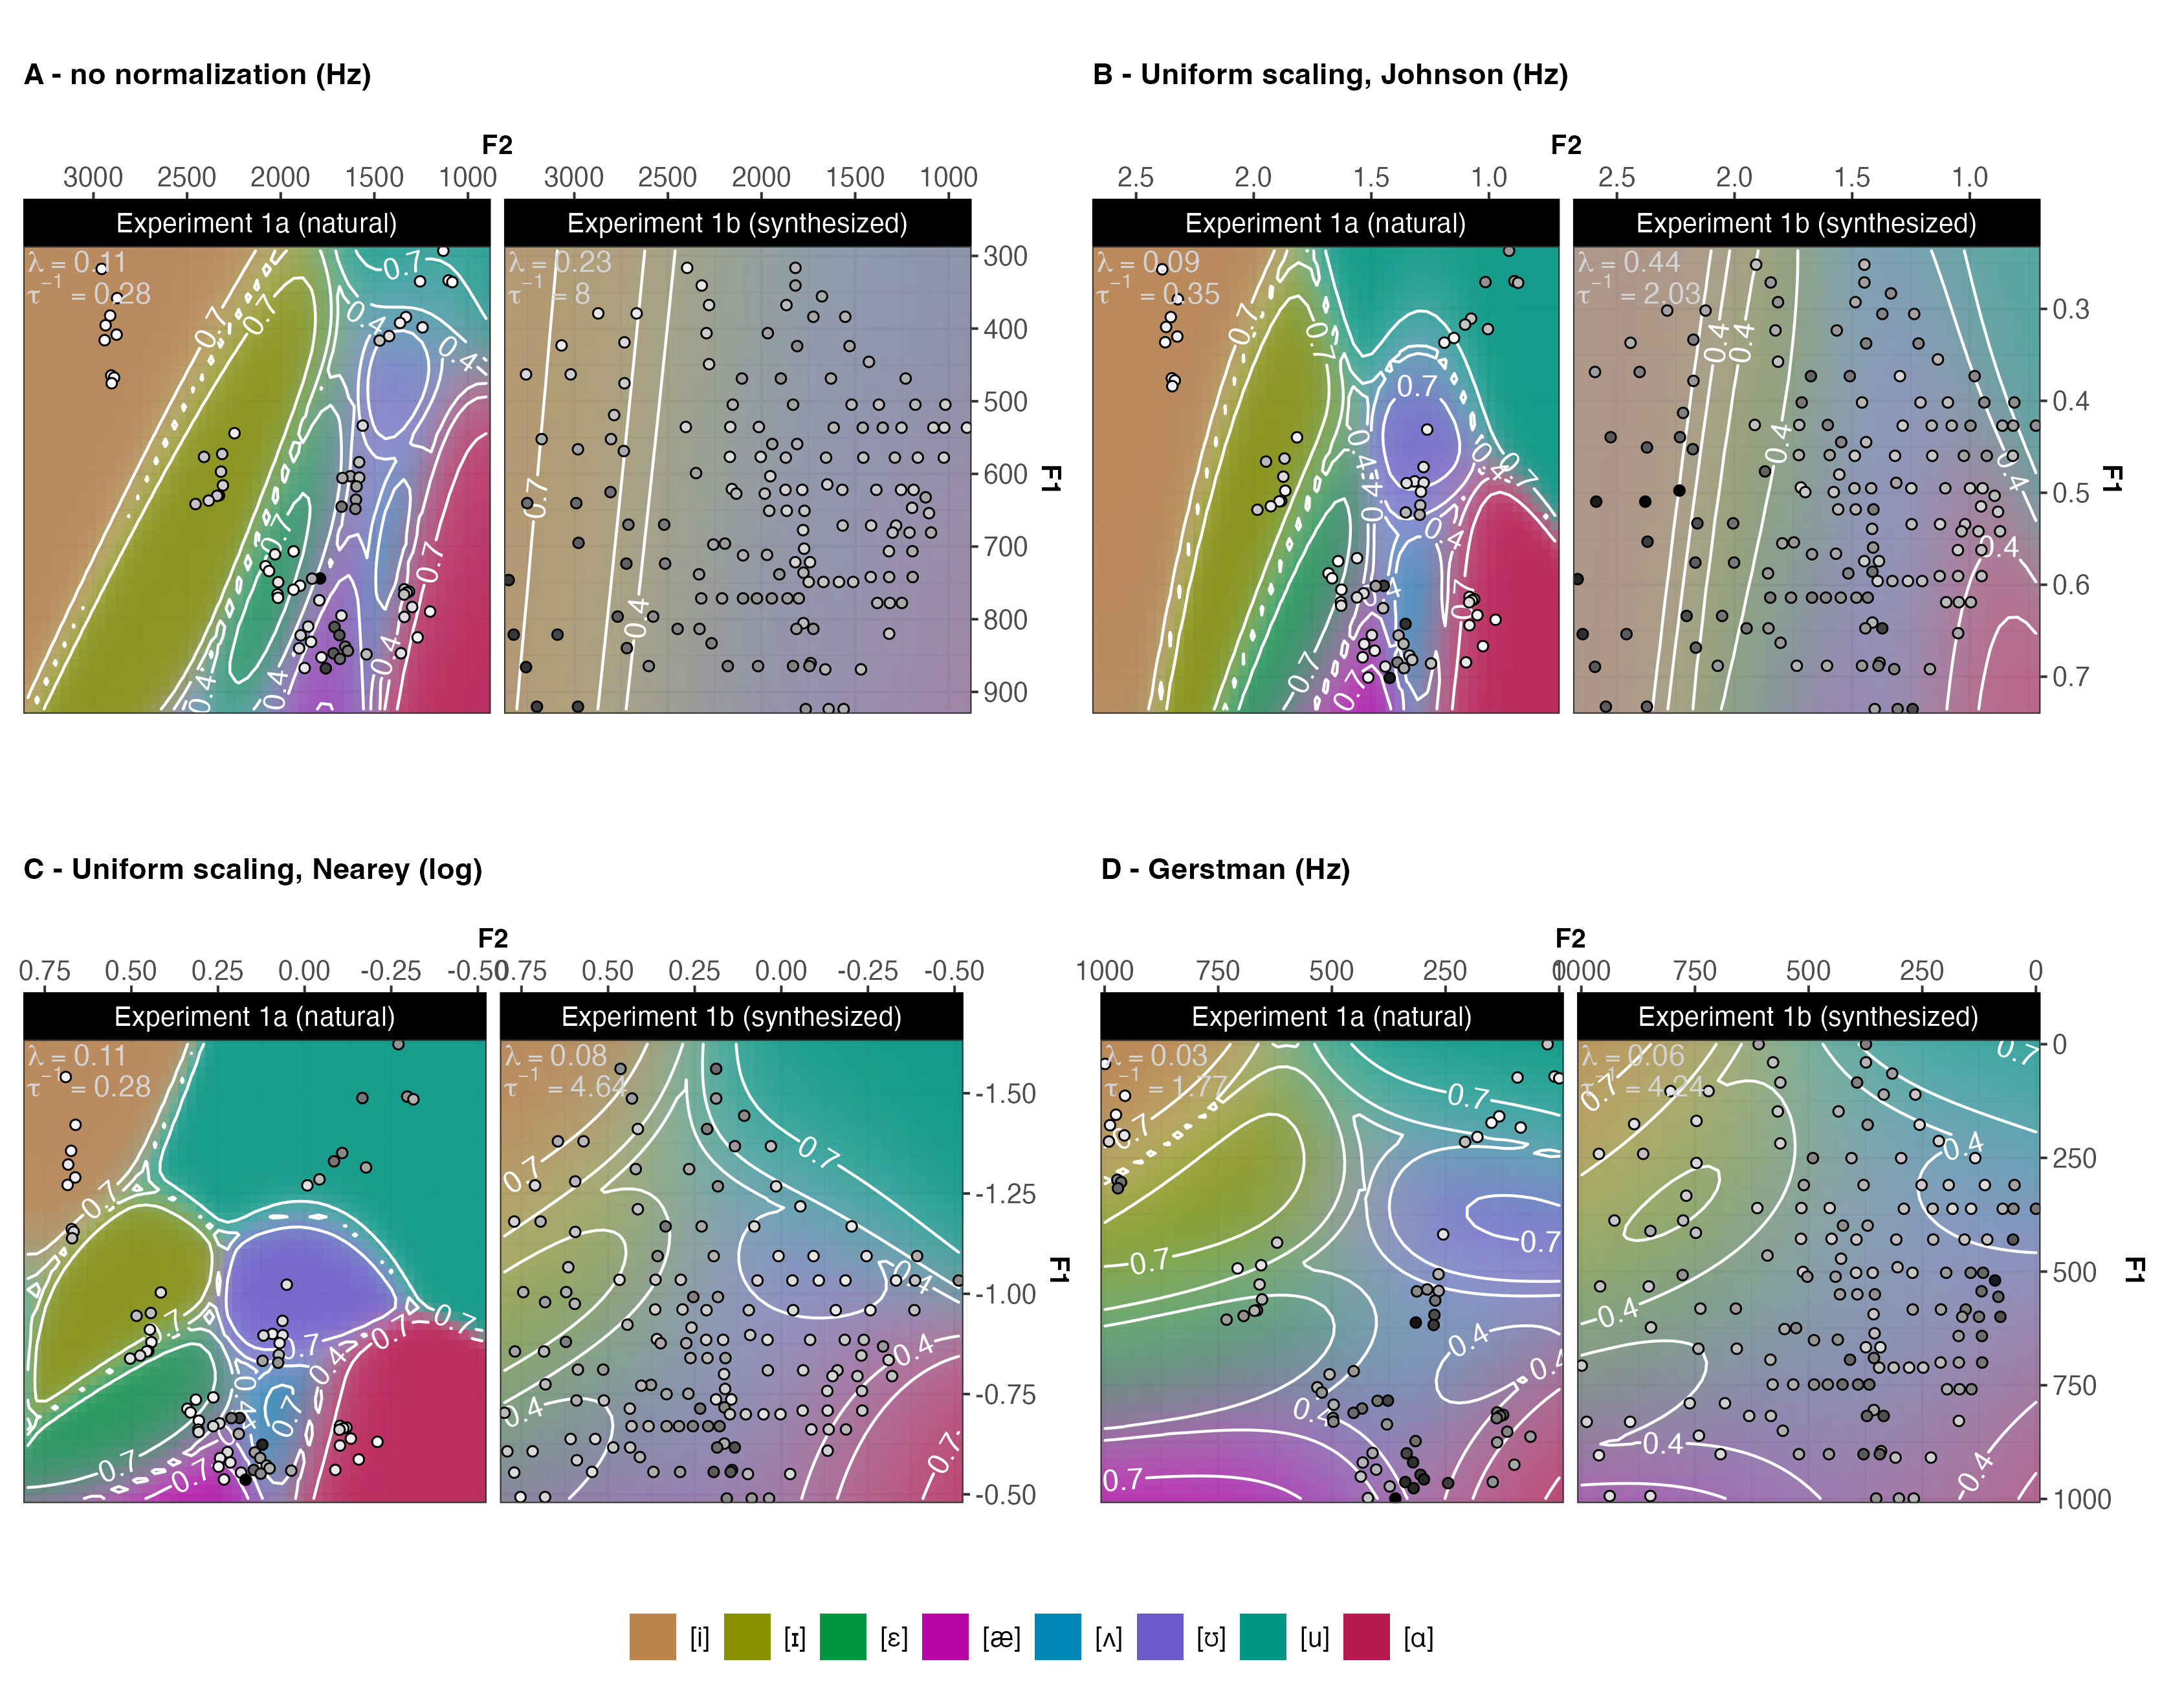
\includegraphics[width=0.8\linewidth]{../../figures/p.prediction-landscapes-study1} 

}

\caption{Predicted categorization functions over the F1-F2 space under four different normalization accounts. For each account, we show the predicted posterior probabilities of all eight vowels obtained by averaging over the maximum likelihood parameterizations (of \(\lambda\) and \(\tau^{-1}\)) for the five training sets (shown at top of each panel). \textbf{Top:} absence of normalization shown for reference. \textbf{2nd row:} the best-fitting account for Experiment 1a. \textbf{3rd row:} the best-fitting account for Experiment 1b (and second best for Experiment 1a). \textbf{Bottom:} the second best-fitting account in Experiment 1b. Contours indicate the highest posterior probability of any vowel. Points indicate location of test stimuli. The increasing opacity of points indicates a worse fit by the account (see text for detail).}\label{fig:prediction-landscapes-optim-io}
\end{figure}

Second, the best-fitting parameters (shown at the top of each panel) were relatively comparable across accounts but differed more substantially across experiments. Specifically, the best-fitting estimates of lapse rates \(\lambda\) were generally comparable across the two experiments (with the exception of Nordström \& Lindblom and Johnson normalization, which exhibited substantially higher lapse rates in Experiment 1b; SI \ref{sec:SI-param-est}). This suggests that participants in both experiments were about equally likely to pay attention to the stimulus. The best-fitting noise ratios \(\tau^{-1}\), however, differed substantially across experiments, and were 9 times larger for Experiment 1b (mean \(\tau^{-1}\) = 4.74, SD = 2.57 across normalization accounts) than for Experiment 1a (mean \(\tau^{-1}\) = 0.52, SD = 0.49). This difference most likely reflects the fact that the synthesized stimuli in Experiment 1b left listeners with substantially more uncertainty about the intended category, as discussed during the description of the experiments.

Since noise is assumed to be independent of category variability \citep[see also][]{feldman2009, kronrod2016}, differences in noise ratios can substantially change the categorization function. This is particularly evident for the accounts that had more variable performance across the two experiments. For example, both Johnson (third row) and Lobanov normalization (fourth row) resulted in very different best-fitting categorization functions for Experiments 1a and 1b.

Third and finally, Figure \ref{fig:prediction-landscapes-optim-io} also shows how well accounts fit listeners' responses for each test stimulus (opaqueness of the black points). This begins to explain \emph{why} some accounts fit listeners' responses in Experiment 1b less well. For example, the Johnson normalization account (third row) predicts the responses to the test stimuli in Experiment 1a well, but fails to predict the responses to the test stimuli in Experiment 1b. This drop in performance seems to be primarily driven by stimuli that are unlikely to be articulated by the same talker (lower left, cf.~dashed line in Figure \ref{fig:human-performance}). This might suggest that this account was over-engineered to explain naturally occurring productions---the type of data, it was originally tested on \citep{johnson2020}. A plausible account of normalization, however, should be able to explain human perception to any type of stimulus, including synthesized stimuli. The SI (\ref{sec:SI-by-item}) presents more detailed by-item comparisons of normalization accounts that might be of interest to some readers.

\section{General discussion}\label{sec:G-D}

Research on vowel normalization has an influential history. Cognitive scientists have long aimed to understand the organization of frequency information in the human brain \citep{stevens-volkmann1940, siegel1965}, and how it helps listeners overcome cross-talker variability in the formant-to-vowel mapping \citep[e.g.,][]{joos1948, fant1975, nordstrom-lindblom1975}. Auditory processes that normalize speech inputs for differences in vocal tract physiology are now recognized to be an integral part of speech perception \citep{mcmurray-jongman2011, johnson-sjerps2021, xie2023}. Here, we set out to investigate what types of computations are implicated in the normalization of the frequency information that plays a critical role in the recognition of vowels.

Our results support three theoretical insights. First, human speech perception draws on more than psycho-acoustic transformations or intrinsic information, in line with previous research on normalization \citep{nearey1989, ladefoged-broadbent1957, adank2004}. Rather, formant normalization seems to involve the estimation and storing of talker-specific formant properties. Second, computationally simple uniform scaling accounts provide the best fit to listeners' responses, suggesting comparatively parsimonious maintenance of talker-specific properties. This replicates and extends previous findings that uniform scaling or similarly simple corrections for vocal tract size provide a better explanation for human perception than more complex extrinsic accounts \citep{barreda2021, richter2017}. It is impossible to rule out more complex approaches to perceptual normalization given the large number of possible alternatives. However, given that uniform scaling provides a parsimonious explanation for human formant normalization, and the current absence of empirical evidence for more complex computations, we submit that researchers ought to adapt uniform scaling as our working hypothesis. Third, the psycho-acoustic representation assumed by different normalization accounts matter, as indicated by the comparison of otherwise computationally similar accounts (e.g.~Nearey's vs.~Johnson's uniform scaling).

These results contribute to a still comparatively small body of work that has evaluated competing normalization accounts against listeners' perception, whereas most previous work evaluates accounts against intended productions. Complementing previous work, we took a broad-coverage approach: the present study compared 20 of the most influential normalization accounts against listeners' perception of \emph{hVd} words with all eight US English monophthongs in both natural and synthesized speech. This contrasts with previous work, which has typically focused on subsets of the vowel system, either using natural \emph{or} synthesized speech, and considering a much smaller subset of accounts (typically 2-3 at a time). By considering a wider range of accounts, a wider range of formant values and vowel categories, and multiple types of speech, we aimed to contribute to a more comprehensive evaluation of competing accounts.

Next, we discuss the theoretical consequences of these findings for research beyond formant normalization. Following that, we discuss limitations of the present work, and how future research might overcome them.

\subsection{Consequences for theories of speech perception and beyond}\label{consequences-for-theories-of-speech-perception-and-beyond}

Understanding the perceptual space in which the human brain represents vowel categories---i.e., the normalized formant space---has obvious consequences for research on speech perception. To illustrate how far reaching these consequences can be, we discuss a few examples. For instance, research on \emph{categorical perception} has found that vowels seem to be perceived less categorically than some types of consonants. Recent work has offered an elegant explanation for this finding: the perception of formants---relevant to the recognition of vowels---might be more noisy than the perception of the acoustic cues that are critical to the recognition of less categorically perceived consonants \citep{kronrod2016}. This is a parsimonious explanation, potentially preempting the need for separate explanations for the perception of different types of phonemic contrasts. Kronrod and colleagues based their argument on estimates they obtained for the relative ratio of meaningful category variability to perceptual noise (\(\tau\), the inverse of our noise ratios, \(\tau^-1\)). Critically, this ratio depends both on (i) the perceptual space in which formants are assumed to be represented (Kronrod at al used Mel-transformed formants), and on (ii) whether the meaningful category variability is calculated prior to, or following, normalization (Kronrod et al assumed the former, which increases estimates of category variability). Our point here is not to cast doubt on the results of \citet{kronrod2016} ---the fact that the best-fitting noise ratios in our study were relatively similar across accounts (while varying across experiments) suggests that the result of Kronrod and colleagues are likely to hold even under different assumptions about (i) and (ii)---but rather to highlight how research on the perception and recognition of vowels depends on assumptions about formant normalization. For example, similar points could be raised about experiments on statistical learning that manipulate formant or other frequency statistics \citep[e.g.,][]{chladkova2017, colby2018, xie2021, wade2007}. Such experiments, too, need to make assumptions about the space in which formants are represented. If these assumptions are incorrect, this can affect whether the experimental manipulations have the intended effects, increasing the chance of null effects or misinterpretation of observed effects.

Understanding the perceptual space in which the human brain represents vowel categories also has consequences for research beyond speech perception, perhaps more so than is sometimes recognized. For instance, in sociolinguistics and related fields, Lobanov remains the norm for representing vowels due to its efficiency in removing cross-talker variability \citep[for review, see][]{adank2004, barreda2021}. However, as shown in the present study, removing cross-talker variability is not the same as representing vowels in the perceptual space that listeners actually employ. Here, we do \emph{not} find Lobanov to describe human perception particularly well. On the contrary, we find no support for the hypothesis that human speech perception employs these more complex computations that have been found to perform best at reducing category variability. This should worry sociolinguists. In order to understand how listeners infer a talker's background or social identity, it is important to understand the perceptual space in which inferences are actually rooted. Critically, the representations resulting from formant normalization presumably form an important part of the information that listeners use to draw social and linguistic inferences. It should thus be obvious that the use of normalization accounts that do not actually correspond to human perception can both mask real markers of social identity, and hallucinate markers that are not actually present. For example, in order to determine how a talker's social identity influences their vowel realizations, it is important to discount \emph{all and only} effects that listeners' will attribute to physiology, rather than social identity \citep{disner1980, hindle1978}.

Similar concerns apply to dialectology, research on language change, second language acquisition research, etc. For example, the perceptual space in which vowels are represented is critical to well-formed tests of hypotheses about the factors shaping the organization of vowel inventories across languages of the world \citep{lindblom1986, stevens1972, stevens1989}. It is essential in testing hypotheses about the extent to which the cross-linguistic realization of those systems is affected by perceptual processes \citep{flemming2010, steriade2001}, or by preferences for communicatively efficient linguistic systems \citep[e.g.,][]{hall2018, lindblom1990, moulin2015}. Similarly, tests of the hypothesis that vowel \emph{articulation} during natural interactions is shaped by communicative efficiency do in obvious ways depend on assumptions about the perceptual space in which talkers---by hypothesis---aim to reduce perceptual confusion \citep[cf.][]{buz-jaeger2016, gahl2012, scarborough2010, wedel2018}. The same applies to any other line of research that aims to understand the perceptual consequences of formant variation across talkers, including research on infant- or child-directed speech \citep{eaves2016, kuhl1997}, and research on whether non-native talkers are inherently more variable than native talkers \citep{smith2019, vaughn2019, xie-jaeger2020}. In short, the perceptual space in which vowels are represented is a critical component of understanding the structure of vowel systems, the factors that shape them, and the ways in which they are used in natural language.

\subsection{Limitations and future directions}\label{limitations-and-future-directions}

The present work shares a few limitations with previous work. Here we focus on limitations that follow from the assumptions we made in our computational framework. While theories and hypotheses often contain substantial vagueness, \emph{quantitative tests} of those theories---as we have done here---require assumptions about \emph{every} aspect of the model. Here, this included all the steps necessary to link properties of the stimuli to listeners' responses. For this purpose, we adopted the ASP framework \citep{xie2023}, and visualized the graphical model that links stimuli (\(x\)) to responses (\(r\)) in Figure \ref{fig:model-perceptual-decision-making}.

Many of the assumptions we made should be quite uncontroversial---e.g., the decision to include both external (environmental) and internal (perceptual) noise in our model. While these noise sources are often ignored in modeling human behavior, it is uncontroversial that they exist. Other assumptions we made were introduced as simplifying assumptions for the sake of feasibility---e.g., we expressed the effect of both types of noise through a single parameter that related the average within-category variability of formants to noise variability in the transformed and normalized formant space. In reality, however, environment noise can have effects that are independent of internal noise, and internal noise likely affects information processing at multiple (or all) of the steps shown in Figure \ref{fig:model-perceptual-decision-making}. Such simplifying assumptions are both inevitable, and not necessarily problematic: as long as they do not introduce systematic bias to the evaluation of normalization accounts, they should not limit the generalizability of our results.

Some of our assumptions, however, might be more controversial. For example, we assumed that category representations can be expressed as multivariate Gaussian distributions in the formant space. This assumption, too, is a simplifying assumption---it simplified the computation of likelihoods---rather than a critical feature of the ASP framework we employed. While human category representations are unlikely to be Gaussians, the alternative, e.g., exemplar representations, would come with its own downsides, such as increased sensitivity to the limited size of phonetic databases and substantial increases in computation time (exemplar representations afford researchers with much larger degrees of freedom). For researchers curious how this and other assumptions we made affect our results, our data and code are shared on OSF. This includes the R markdown document that generates this PDF, making it comparatively easy to revisit any of our assumptions to then regenerate the entire study with a click of a button in RStudio.

Like previous work, we further assumed that all listeners in our experiments use the same underlying vowel representations---the same dialect template(s). However, as already discussed, it is rather likely that not all of our listeners employed the same dialect template(s). An additional analysis reported in the SI (\ref{sec:SI-dialect-subset}) thus compared normalization accounts against only the subset of listeners who employed the dialect template used by the majority of participants (see lower-left of Figure \ref{fig:human-confusion}B). This left only 11 participants for Experiment 1a (61.1\%) and 14 for Experiment 1b (77.8\%), substantially reducing statistical power. Replicating the main analysis, uniform scaling accounts again fit listeners' behavior well across both experiments. The best-performing accounts did, however, differ from the ones obtained for the superset of data (see SI, \ref{sec:SI-dialect-subset}).

A related assumption was introduced by the use of a phonetic database to approximate listeners' vowel representations. This deviates from most previous evaluations of normalization accounts \citetext{\citealp{mcmurray-jongman2011}; \citealp{barreda2021}; \citealp[but see][]{richter2017}}, and reflects our commitment to a strong assumption made by most theories of speech perception: that listeners' representations reflect the formant statistics previously experienced speech input. By using a phonetic database to estimate listeners' representations, we \emph{substantially} reduced the degrees of freedom in the evaluation of normalization accounts, reducing the chance of over-fitting to the data from our experiments. Our approach does, however, also introduce two new assumptions.

First, our approach assumes that the mixture of dialect template(s) used by talkers in the database sufficiently closely approximates those of the listeners in our experiments. Some validation for this assumption comes from the additional analysis reported in the preceding paragraph: when we subset listeners to only those who used the majority dialect template, this improved the fit of all normalization accounts---as expected, if the category representations we trained on the phonetic database primarily reflect those listeners' representations (see SI, \ref{sec:SI-dialect-subset}). Future work could further address this assumption in a number of ways. On the one hand, dialect analyses like the ones we presented for our listeners (in Figure \ref{fig:human-confusion}B) could compare listeners' templates against the templates used by talkers in the database. Alternatively or additionally, researchers could see whether our results replicate if ideal observers are instead trained on other databases that have been hypothesized to reflect a `typical' L1 listeners' experience with US English.

Second, we made the simplifying assumption that listeners' category representation---or at least the representations listeners' drew on during the experiment---are talker-\emph{independent} (we trained a single set of multivariate Gaussian categories, rather than, e.g., hierarchically organized set of multiple dialect templates). While this assumption is routinely made in research on normalization and beyond, it might well be wrong \citep[see e.g.,][]{xie2021}.

Finally, the evaluation of normalization accounts in the present work shares with all previous work \citep[e.g.,][]{apfelbaum-mcmurray2015, cole2010, mcmurray-jongman2011, barreda2021, nearey1989, richter2017} another simplifying assumption that is clearly wrong: the assumption that listeners \emph{know} the talker-specific formant properties required for normalization. Specifically, we normalized the input for each ideal observer using the maximum likelihood estimates of the normalization parameters for the respective experiment. For example, for the evaluation of the ideal observer trained on Lobanov normalized formants against listeners' responses in Experiment 1a, we used the formant means and standard deviations of the stimuli used in Experiment 1a to normalize F1 and F2. While this follows previous work, it constitutes a problematic assumption for the evaluation of extrinsic normalization accounts. For these accounts, the approach adopted essentially assumes the ability to predict the future: even on the first trial of the experiment, the input to the ideal observers were formants that were normalized based on the maximum likelihood estimate of the normalization parameters given the acoustic properties of \emph{all} stimuli. Listeners instead need to \emph{incrementally infer} talker-specific properties from the speech input \citep{nearey-assmann2007, xie2023}. The development and testing of incremental variants of formant normalization strikes us an important avenue for future research.

\subsection{Concluding remarks}\label{concluding-remarks}

We set out to compare how well competing accounts of formant normalization explain listeners' perception of vowels. We developed a computational framework that makes it possible to compare a large number of different accounts against multiple data sets. The code we share on OSF makes it possible to `plug in' different accounts of vowel normalization, different phonetic databases, and different perception experiments. This, we hope, will substantially reduce the effort necessary to conduct similar evaluations on other datasets, dialects, and languages.

Comparing 20 of the most influential normalization accounts against L1 listeners' perception of US English monophthongs, we found that the normalization accounts that best describe listeners' perception share that they (1) learn and store talker-specific properties and (2) that they seem to be computationally very simple---taking advantage of the physics of sound generation to use as few as a single parameter to normalize inter-talker variability in vocal tract size. While the number of studies that have compared normalization accounts against \emph{listeners'} behavior remains surprisingly small, these two results confirm the findings from more targeted comparisons that were focused on 2-3 accounts at a time \citep{barreda2021, nearey1989, richter2017}. Overall then, we submit that it is time for research in speech perception and beyond to consider simple uniform scaling the most-likely candidate for human formant normalization.

\begin{acknowledgments}
Earlier versions of this work were presented at 2023 ASA meeting, ExLing 2022, at the Department of Computational Linguistics at the University of Zürich and at the Department of Swedish language and multilingualism at Stockholm University. We are grateful to OMITTED FOR REVIEW.
\end{acknowledgments}

\section*{Author Contributions}\label{author-contributions}
\addcontentsline{toc}{section}{Author Contributions}

AP designed the experiments and collected the data, with input from TFJ. TFJ programmed the experiments with input from AP. AP analyzed the experiments, with input from TFJ. AP and TFJ wrote the code to implement and fit the normalization models, with input from SB. AP developed the visualizations within input from SB and TFJ. AP wrote the first draft of the manuscript with edits by SB and TFJ.

\section*{Author Declarations}\label{author-declarations}
\addcontentsline{toc}{section}{Author Declarations}

\subsection*{Conflict of Interest}\label{conflict-of-interest}
\addcontentsline{toc}{subsection}{Conflict of Interest}

The authors declare that the research was conducted in the absence of any commercial or financial relationships that could be construed as a potential conflict of interest.

\subsection*{Ethics approval}\label{ethics-approval}
\addcontentsline{toc}{subsection}{Ethics approval}

This study was reviewed and approved Research Subjects Review Board (RSRB) of the University of Rochester (STUDY00000417) under the OHSP and UR policies, and in accordance with Federal regulation 45 CFR 46 under the university's Federal-wide Assurance (FWA00009386).

\newpage

\section*{\texorpdfstring{Supplementary information for \emph{Persson, Barreda \& Jaeger (2024). Comparing accounts of formant normalization against US English listeners' vowel perception}}{Supplementary information for Persson, Barreda \& Jaeger (2024). Comparing accounts of formant normalization against US English listeners' vowel perception}}\label{supplementary-information-for-persson-barreda-jaeger-2024.-comparing-accounts-of-formant-normalization-against-us-english-listeners-vowel-perception}
\addcontentsline{toc}{section}{Supplementary information for \emph{Persson, Barreda \& Jaeger (2024). Comparing accounts of formant normalization against US English listeners' vowel perception}}

\singlespacing

\setcounter{page}{1}
\setcounter{section}{0}
\setcounter{footnote}{0}
\setcounter{figure}{0}
\setcounter{table}{0}
\setcounter{equation}{0}

\renewcommand{\thesection}{\S \arabic{section}}
\renewcommand{\thefootnote}{S\arabic{footnote}}
\renewcommand{\thefigure}{S\arabic{figure}}
\renewcommand{\thetable}{S\arabic{table}}
\renewcommand{\theequation}{S\arabic{equation}}

\renewcommand{\theHsection}{S\arabic{section}}
\renewcommand{\theHfootnote}{S\arabic{footnote}}
\renewcommand{\theHfigure}{S\arabic{figure}}
\renewcommand{\theHtable}{S\arabic{table}}
\renewcommand{\theHequation}{S\arabic{equation}}

\section{Required software}\label{sec:SI-software}

Both the main text and these supplementary information (SI) are derived from the same R markdown document available via \href{OSF}{https://osf.io/zemwn/}. It is best viewed using Acrobat Reader. The document was compiled using \texttt{knitr} in RStudio with R:

\begin{verbatim}
##                _                           
## platform       aarch64-apple-darwin20      
## arch           aarch64                     
## os             darwin20                    
## system         aarch64, darwin20           
## status                                     
## major          4                           
## minor          4.0                         
## year           2024                        
## month          04                          
## day            24                          
## svn rev        86474                       
## language       R                           
## version.string R version 4.4.0 (2024-04-24)
## nickname       Puppy Cup
\end{verbatim}

Readers interested in working through the R markdown, and knitting it into a PDF will also need to download the IPA font \href{https://software.sil.org/doulos/download/}{SIL Doulos} and a Latex environment like (e.g., \href{https://tug.org/mactex/mactex-download.html}{MacTex} or the R library \texttt{tinytex}).

We used the following R packages to create this document: R \citep[Version 4.4.0;][]{R-base} and the R-packages \emph{assertthat} \citep[Version 0.2.1;][]{R-assertthat}, \emph{brms} \citep[Version 2.21.0;][]{R-brms_a, R-brms_b, R-brms_c}, \emph{Cairo} \citep[Version 1.6.2;][]{R-Cairo}, \emph{cmdstanr} \citep[Version 0.7.1;][]{R-cmdstanr}, \emph{dplyr} \citep[Version 1.1.4;][]{R-dplyr}, \emph{ellipse} \citep[Version 0.5.0;][]{R-ellipse}, \emph{forcats} \citep[Version 1.0.0;][]{R-forcats}, \emph{furrr} \citep[Version 0.3.1;][]{R-furrr}, \emph{fuzzyjoin} \citep[Version 0.1.6;][]{R-fuzzyjoin}, \emph{ggforce} \citep[Version 0.4.2;][]{R-ggforce}, \emph{ggh4x} \citep[Version 0.2.8;][]{R-ggh4x}, \emph{ggnewscale} \citep[Version 0.4.10;][]{R-ggnewscale}, \emph{ggplot2} \citep[Version 3.5.1;][]{R-ggplot2}, \emph{ggtext} \citep[Version 0.1.2;][]{R-ggtext}, \emph{knitr} \citep[Version 1.47;][]{R-knitr}, \emph{linguisticsdown} \citep[Version 1.2.0;][]{R-linguisticsdown}, \emph{lubridate} \citep[Version 1.9.3;][]{R-lubridate}, \emph{magrittr} \citep[Version 2.0.3;][]{R-magrittr}, \emph{mgcv} \citep[Version 1.9.1;][]{R-mgcv_a, R-mgcv_b, R-mgcv_c, R-mgcv_d}, \emph{modelr} \citep[Version 0.1.11;][]{R-modelr}, \emph{MVBeliefUpdatr} \citep[Version 0.0.1.10;][]{R-MVBeliefUpdatr}, \emph{nlme} \citep[Version 3.1.164;][]{R-nlme}, \emph{patchwork} \citep[Version 1.2.0;][]{R-patchwork}, \emph{phonR} \citep[Version 1.0.7;][]{R-phonR}, \emph{phonTools} \citep[Version 0.2.2.2;][]{R-phonTools}, \emph{plotly} \citep[Version 4.10.4;][]{R-plotly}, \emph{purrr} \citep[Version 1.0.2;][]{R-purrr}, \emph{Rcpp} \citep[Version 1.0.12;][]{R-Rcpp}, \emph{readr} \citep[Version 2.1.5;][]{R-readr}, \emph{remotes} \citep[Version 2.5.0;][]{R-remotes}, \emph{RJ-2021-048} \citep{R-RJ-2021-048}, \emph{rlang} \citep[Version 1.1.4;][]{R-rlang}, \emph{stringr} \citep[Version 1.5.1;][]{R-stringr}, \emph{tibble} \citep[Version 3.2.1;][]{R-tibble}, \emph{tidybayes} \citep[Version 3.0.6;][]{R-tidybayes}, \emph{tidyr} \citep[Version 1.3.1;][]{R-tidyr}, and \emph{tidyverse} \citep[Version 2.0.0;][]{R-tidyverse}.

If opened in RStudio, the top of the R markdown document should alert you to any libraries you will need to download, if you have not already installed them. The full session information is provided at the end of this document.

\subsection{Interested in using R markdown do create APA formatted documents that integrate your code with your writing?}\label{interested-in-using-r-markdown-do-create-apa-formatted-documents-that-integrate-your-code-with-your-writing}

A project template, including R markdown files that result in APA-formatted PDFs, is available at \url{https://github.com/hlplab/template-R-project}. Feedback is welcome by the contact author for this paper or \href{mailto:fjaeger@ur.rochester.edu}{\nolinkurl{fjaeger@ur.rochester.edu}}. We aim to help others avoid the detours we made when first deciding to embrace literal coding to increase transparency in our projects.

\section{Additional information in Experiments 1a and 1b}\label{additional-information-in-experiments-1a-and-1b}

\subsection{Exclusions}\label{sec:SI-exclusions}

We first applied trial-level exclusion criteria to each participant, and then applied participant-level exclusion criteria.

\subsubsection{Trial exclusions}\label{trial-exclusions}

We excluded trials with RTs more than 3 standard deviations faster or slower than expected. This was determined by first z-scoring the log-transformed RTs \emph{within each participant} (by subtracting the participants' mean from each observation and dividing through the participants standard deviation) and then z-scoring these z-scores \emph{within each trial} across participants. This double-scaling approach was necessary as participants' RTs decreased substantially over the first few trials and then continued to decrease less rapidly until converging against a participant-specific minimum. This criterion did not remove just the first few trials but rather removed RTs that were unusually fast or slow \emph{for that participant at that trial}. And, unlike more complicated methods (like developing a model of cross-trial decreases in RTs), the approach employed here does not make any assumptions about the shape of the speed up in RTs across trials. In total, 41 trials were excluded from Experiment 1a, and 76 from Experiment 1b.

\subsubsection{Participant exclusion}\label{participant-exclusion}

Participants were excluded if they (1) failed to pay attention to the instruction to wear over-the-ear-headphones, (2) had unusually slow or fast RT-means compared to other participants (more than 3 standard deviations faster or slower in their mean log-transformed RTs compared to other participants), (3) clearly did not do the task (e.g., randomly clicking on different response options). Finally, participants were excluded if (4) the trial-level exclusions removed too many trials (\textgreater20\% of all trials).

For Experiment 1a, 1 participant was excluded based on the first criteria, as s/he used external speakers instead of head set (based on response in post-experiment questionnaire). One additional participant was excluded based on the second criterion. For Experiment 1b, no participants were excluded based on criteria 1 and 2.

As the experiments did not contain catch trials, we visualized participants' individual responses in order to identify participants that answered randomly, independent of the stimulus (third criterion). For Experiment 1a, Figure \ref{fig:SI-exp1a-responses} suggests that 4 participants did not perform the task. This includes \emph{had} responses to stimuli located across the entire vowel space, \emph{heed} responses to stimuli located in the low back part of the space, or \emph{odd} responses to stimuli located in the high front part of the space. For Experiment 1b, Figure \ref{fig:SI-exp1b-responses} suggests that 2 participants displayed unusual response patterns, responding \emph{who'd} or \emph{hod} for tokens in the high front part of the space, and \emph{heed} for tokens in the high center and back parts.

Finally, no participant was excluded based on the forth criteria (too many missing trials). In total, 6 participants were excluded from Experiment 1a (one of these were excluded based on multiple criteria), and 2 participants were excluded from Experiment 1b. This left 18 participants for Experiment 1a, and 22 participants for Experiment 1b.





\begin{figure}[!ht]

{\centering \includegraphics[width=0.9\linewidth]{../../figures/knitted/SI-exp1a-responses} 

}

\caption{Participants' response patterns in Experiment 1a. Color and vowel label indicate response provided by participants on each test location. Each vowel was repeated twice. Participants that displayed unusual response patterns and were therefore excluded, are highlighted.}\label{fig:SI-exp1a-responses}
\end{figure}

\begin{figure}[!ht]

{\centering \includegraphics[width=0.9\linewidth]{../../figures/knitted/SI-exp1b-responses} 

}

\caption{Participants' response patterns in Experiment 1b. Color and vowel label indicate response provided by participants on each test location. Each vowel was repeated twice. Participants that displayed unusual response patterns and were therefore excluded, are highlighted.}\label{fig:SI-exp1b-responses}
\end{figure}

\subsection{Distribution of stimuli F1-F3 in Experiments 1a and 1b}\label{distribution-of-stimuli-f1-f3-in-experiments-1a-and-1b}

The main text provides visualization of the stimuli's F1 and F2. Figure \ref{fig:SI-plot-cues-3d} shows the same stimuli in the 3D space defined by F1-F3. In addition, the F3 values in each synthesized token was set based on the F1-F2 values of the stimuli. Specifically, we used a linear regression based on the stimuli in Experiment 1a (predicting F3 from F1, F2 and their interaction) to predict F3 values for each F1-F2 combination in Experiment 1b. This difference in F3-distributions between experiment stimuli is clearly visible in Figure \ref{fig:SI-plot-cues-3d}\textbf{(b)}.

Figure \ref{fig:SI-plot-cues-3d}\textbf{(b)} further suggests that the talker used in Experiment 1a seems to produce some of the low (and high) back vowels with higher F3 values than might be expected. If this talker's F3-distribution is indeed unexpected or unusual (in comparison to listeners' expectations or to other talkers in the database), this could potentially partly explain the decrease in model fit for some of the normalization models when fit to F1-F3 compared to F1-F2 (see Section \ref{sec:SI-F1F3}).



\begin{figure}

{\centering \subfloat[Looking at F1 and F2 (F3 is depth). This perspective illustrates that the stimuli of Experiment 1b spanned a much larger part of the F1-F2 space.\label{fig:SI-plot-cues-3d-1}]{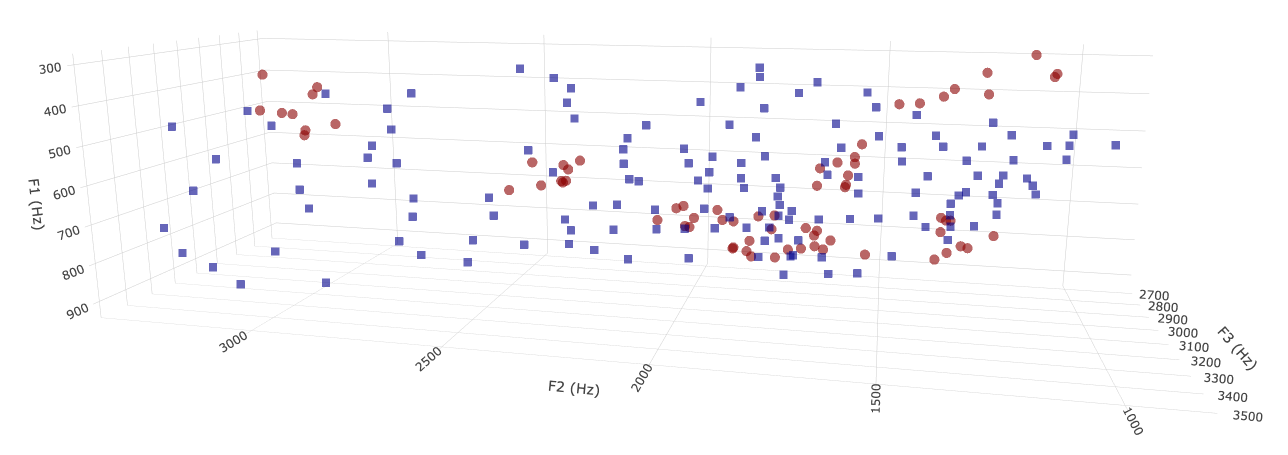
\includegraphics[width=0.6\linewidth]{figures/p.3Dcues.1} }\newline\subfloat[Looking at F2 and F3 (F1 is depth). This perspective illustrates differences in the distribution of F3 across the two experiments. In Experiment 1b, F3 was synthesized to follow a linear function of F1 and F2, fit based on the stimuli from Experiment 1a. This perspective also illustrates that some stimuli of Experiment 1a had much higher or lower F3 than expected based on their F1 and F2 (under the assumption of a linear relation).\label{fig:SI-plot-cues-3d-2}]{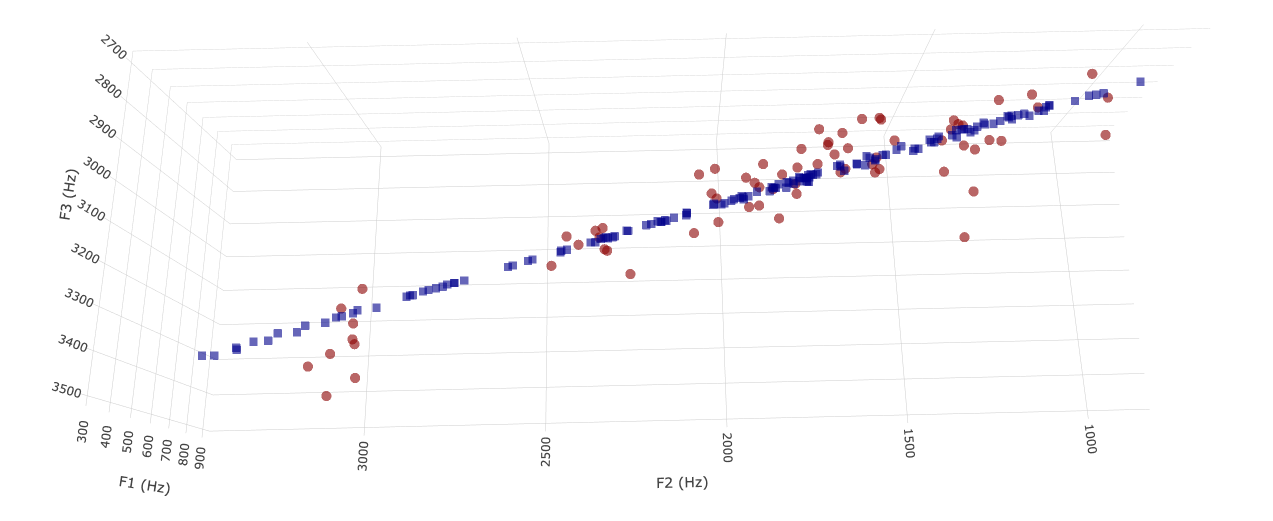
\includegraphics[width=0.6\linewidth]{figures/p.3Dcues.2} }\newline

}

\caption{Stimuli of Experiments 1a (\textbf{red circles}) and 1b (\textbf{blue squares}) in F1-F3 space. Shown are three different perspectives on the same data.}\label{fig:SI-plot-cues-3d}
\end{figure}

\subsection{Auxiliary analysis of participant responses in Experiments 1a and 1b}\label{sec:SI-aux-entropy}

Participants in Experiment 1b showed overall less agreement in their responses to the stimuli than participants in Experiment 1a, as indicated by the higher response entropy in Experiment 1b. As stated in the main text, response entropies differed even for tokens that were acoustically similar and only differed in \(\le 30\) Hz along F1 and F2. Figure \ref{fig:SI-overlap-tokens} visualizes differences in categorization behavior for these 40 acoustically similar tokens. For some of these tokens, participants selected the same category across experiments. However, even when selecting the same response option, participants still displayed higher disagreement for the tokens in Experiment 1b (mean by-item response entropy for the overlapping tokens in Experiment 1a = 0.18 bits, SE = 0.03; and for the overlapping tokens in Experiment 1b = 0.39 bits, SE = 0.03).



\begin{figure}

{\centering \includegraphics[width=0.8\linewidth]{../../figures/knitted/SI-overlap-tokens} 

}

\caption{Listeners' categorization responses in Experiments 1a and 1b, for comparable tokens in Hertz space. The vowel label indicates the most frequent response provided by participants on each test location. Size indicates how consistent responses were across participants, which larger symbols indicating more consistent responses (lower entropy).}\label{fig:SI-overlap-tokens}
\end{figure}

To investigate the extent to which these differences in response entropy could be explained by differences in stimuli characteristics, we fit a series of general additive models (GAM). First, we confirmed that the difference in response entropy between experiments across all tokens was indeed statistically significant, by regressing response entropy against experiment (treatment coded; \(p < .0001\), deviance explained = 43.8\%). Next, we fit the same model to a subset of the data that excluded all \emph{hut} and \emph{odd} responses from Experiment 1a. This was done in order to assess whether differences in lexical context contributed to differences in entropy between experiments. This model confirmed that differences in entropy could not be reduced to differences in lexical context, since experiment remained a significant predictor of response entropy (\(p < .0001\), deviance explained = 31.7\%).

In order to determine the extent to which this difference between experiments can be explained by differences in formants, we fit additional GAMs to the same subset. First, we regressed response entropy against both experiment and a tensor smooth of F1, F2, and F3. The tensor smooth allows for non-linear effects of, and interactions between, formants. To be maximally conservative, we normalized formants using one of the accounts that our computational studies find to be the best fit against human responses (Nearey's uniform scaling). The GAM with both formants and experiment explained 78.7\% of the deviance in response entropy. Experiment still was a significant predictor of response entropy, suggesting that the difference in response entropy between experiments is not solely due to differences in formants. Formants did, however, explain a substantial amount of the difference in response entropy between experiments: a GAM with just the tensor smooth of F1-F3 explained 70.8\% of the deviance.

Experiment thus explained at least 7.9\% of the deviance when it was added to this model---about 24.9\% of the deviance explained if \emph{only} experiment is included in the model (31.7\%). These informal comparisons suggest that up to about two thirds of the deviance that is explained by experiment is due to differences in formants between the experiments.
Results using unnormalized formants confirmed these results (but, as expected if uniform scaling is approximates the normalization employed by listeners, uniformly scaled formants explained about 4\% more variance in response entropy).

\section{Additional information on the computational comparison of normalization accounts}\label{additional-information-on-the-computational-comparison-of-normalization-accounts}

\subsection{Methods}\label{methods-1}

\subsubsection{\texorpdfstring{Vowel data used to train ideal observers \citep{xie-jaeger2020}}{Vowel data used to train ideal observers {[}@xie-jaeger2020{]}}}\label{sec:SI-xie-jaeger}

We provide additional information on the formant data from the \citet{xie-jaeger2020} database that we used to train the ideal observers, as described in the main text. The database consists of 1168 \emph{hVd} word recordings from 16 (5 female) L1 talkers of a Northeastern dialect of US English (ages 18 to 35 years old). The talkers were recorded reading a list of 180 English monosyllabic words, a list of short sentences, and a list of ten \emph{hVd} words---the eight US English monophthongs as well as \emph{aid} and \emph{owed} \citep[for further information, see][]{xie-jaeger2020}. For each talker, the database contains 9-10 recordings of each \emph{hVd} word. An automatic aligner \citep[Penn Phonetics Lab Forced Aligner,][]{yuan2008} was used to obtain estimates for word and segment boundaries.\footnote{We thank Xin Xie and Leslie Li for providing us with the recordings and aligned Praat textgrids.}

The first author manually corrected the automatic alignments for all vowel segmentations. We then used the Burg algorithm in Praat \citep{boersma-weenink2022} to extract estimates of the first three formants (F1-F3) at three time points of the vowel (35, 50, and 65 percent into the vowel). The following parameterization of the Burg algorithm was used:

\begin{itemize}
\tightlist
\item
  Time step (s): 0.01
\item
  Max. number of formants: 5
\item
  Formant ceiling (Hz): 5500 (5000 for the male talkers)
\item
  Window length (s): 0.025
\item
  Pre-emphasis from (Hz): 50
\end{itemize}

In addition to F1-F3, we automatically extracted vowel duration and the fundamental frequency (F0) across the entire vowel. Figure \ref{fig:SI-eng-vowels-all-cues}, adapted from \citet{persson-jaeger2023}, visualizes the vowel data from the \citet{xie-jaeger2020} database for all pairwise combinations of F0, F1, F2, F3 and vowel duration, in raw Hz. Unsurprisingly, the densities along the diagonal suggest that F1 and F2 carry most information for vowel category identity, as indicated by higher between-category separation than the other cues. We also note that there seems to be one female talker with substantially higher F0 and higher formants than the other female talkers.

Figure \ref{fig:SI-eng-vowels-normalized}, adapted from \citet{persson-jaeger2023}, shows the distribution of F1 and F2 in the different normalization spaces used in the main paper. We make a few observations. First, transforming the space into a perceptual scale (\textbf{grey panels}) does not seem to affect the vowel distributions much. Second, intrinsic normalization both increase category separability and more strikingly warps the space. Third, extrinsic centering and standardizing normalization seem to reduce category variability and increase separability, though it is not visually obvious which type of account achieves better separability.



\begin{figure}[!ht]

{\centering \includegraphics[width=1\linewidth]{../../figures/knitted/SI-eng-vowels-all-cues} 

}

\caption{The pairwise distributions of F0, F1, F2, F3, and duration for all 1168 recordings of the eight monophthong \emph{hVd} words in \citet{xie-jaeger2020}. Note that axis directions are not reversed (unlike for the F1-F2 plots in the main text and SI). \textbf{Panels on diagonal:} marginal cue densities of all five cues. \textbf{Lower off-diagonal panels:} each point corresponds to a recording, averaged across the three measurement points within each vowel segment. Vowel labels indicate category means across talkers. Male talkers' vowels are boldfaced. \textbf{Upper off-diagonal panels:} Same data as in the lower off-diagonal panels but showing ellipses for bivariate Gaussian 95\% probability mass around category means.}\label{fig:SI-eng-vowels-all-cues}
\end{figure}



\begin{figure}

{\centering \includegraphics[width=1\linewidth]{../../figures/knitted/SI-eng-vowels-normalized} 

}

\caption{The 8 monophthong vowels of US English from the \citet{xie-jaeger2020} database when F1 and F2 are transformed into a perceptual scale (\textbf{grey}), intrinsically normalized (\textbf{yellow}), or extrinsically normalized through centering (\textbf{blue}) or standardizing (\textbf{purple}). Each point corresponds to one recording, averaged across the three measurement points within each vowel segment. Shape indicates gender (female talkers represented by points, male talkers by triangles).}\label{fig:SI-eng-vowels-normalized}
\end{figure}

\subsubsection{\texorpdfstring{Normalization parameters \(\theta\)}{Normalization parameters \textbackslash theta}}\label{sec:SI-norm-params}

Figure \ref{fig:SI-norm-params} relates the normalization parameters \(\theta\) obtained for each experiment to those obtained for the five training sets of the \citet{xie-jaeger2020} database. This comparison serves two purposes. First, by comparing the \(\theta\) of Experiment 1a, which was based on natural productions, to the \(\theta\)s obtained from \citet{xie-jaeger2020}, we can assess the extent to which the talker used for Experiment 1a is `typical' relative to the other talkers of that database. Second, by comparing the range and variability of the \(\theta\) across normalization accounts and experiments, we hope to provide readers with intuitions about differencves in the volatility of different types of parameters, and assess the difference between the beliefs the ideal observers have about the parameters and the parameters in the experiment stimuli.

Figure \ref{fig:SI-norm-params} suggests that the talker used in Experiment 1a is overall aligned with the other talkers in the database, as indicated by the relative distance between the blue dots to the horizontal dotted line. How closely the estimates obtained from the talker in Experiment 1a match the estimates obtained from the other talkers depend on the \(\theta\) assumed. For instance, for accounts assuming separate parameters for each formant, \(\theta\)s for F2 seem to be a closer match than \(\theta\)s for F1, with the exceptions of Gerstman's maxima and Lobanov's SD.

Figure \ref{fig:SI-norm-params} further indicates that the reliability by which the formant statistics can be established for the same amount of data, seems to depend on the perceptual space assumed by the normalization account. For instance, parameters in Hertz space display more variability. Comparing between accounts assuming the same perceptual space, we also note that some parameters are more variable than others. For instance, mean estimates display less variability than estimates of SD, and range values (minima and maxima)---i.e., the parameters employed by standardizing accounts. Range values and SDs also differ more between experiments than other estimates. This is expected given that the stimuli in Experiment 1b sampled larger parts of the phonetic space (see Section \ref{sec:stimuli}). Finally, estimates of SDs and range values also seem to differ more between the phonetic database and the two experiments.



\begin{figure}

{\centering \includegraphics[width=0.9\linewidth]{../../figures/knitted/SI-norm-params} 

}

\caption{Comparing normalization parameters \(\theta\) across the phonetic database used to estimate listeners' prior experience \citep{xie-jaeger2020} and Experiments 1a and 1b. Only accounts that assume talker-specific normalization parameters are shown. Dotted line indicates identical \(\theta\) estimates for the phonetic database and experiment stimuli.}\label{fig:SI-norm-params}
\end{figure}

\subsubsection{Optimization process to fit models to human responses}\label{sec:SI-optim-process}

To determine the best-fitting values for the two degrees of freedom---lapse rate (\(\lambda\)) and noise ratio (\(\tau^{-1}\))---when fitting the ideal observers to listeners' responses in Experiment 1a and 1b, we used constrained quasi-Newton optimization \citep{byrd1995}. Optimization was performed separately for each of the 200 combinations of normalization account, experiment, and training set. Specifically, we maximized the \emph{likelihood} of the human categorization responses in each experiment under the categorization model conditional on the model's lapse rate and noise, \(\Sigma_i^N \log p(response_i | F1_{i,\theta}, F2_{i,\theta}, M_{\theta, \lambda, \Sigma_{noise}})\), where \(response_i\) is the \(i\)th categorization response, \(F1_{i,\theta}, F2_{i,\theta}\) are the F1 and F2 values for the \(i\)th observation after normalization (with parameters \(\theta\) being estimated based on the distribution of phonetic cues across the stimuli in the experiment). \(M_{\theta, \lambda, \Sigma_{noise}}\) is the categorization model in Figure \ref{fig:model-perceptual-decision-making}, with normalization parameters \(\theta\) fixed based from the prior cue distribution in the phonetic database \citep{xie-jaeger2020}, and \(\lambda\) and \(\tau^{-1}\) as the only free parameters to maximize the likelihood. The best-fitting parameterizations were determined by means of the \texttt{optim()} function in \texttt{R}'s \texttt{stats} package \citep{R-base}. The starting value of lapse rates and noise were set to 0.1 and 0.15, respectively. We set the lower and upper bounds to \ensuremath{10^{-10}} \(\geq\) lapse rate \(\geq\) 1, and \ensuremath{10^{-10}} \(\geq\) noise \(\geq\) 10 \citep[i.e., including values well beyond previously observed estimates for perceptual noise in][p.~1698]{kronrod2016}.

Section \ref{sec:SI-study1-grid-search} presents additional analyses that instead used a grid search over the parameter space. These analyses overall confirm the results presented in the main text.

\subsection{Results for F1-F2}\label{results-for-f1-f2}

\subsubsection{Significance test of model performance}\label{sec:SI-sign-test}

To assess whether normalization significantly improved the fit to listeners' responses, we conducted paired one-sided \emph{t}-tests comparing the maximum likelihood values (averaged across the five training sets) for each normalization account against those in the absence of normalization (dummy coded with the unnormalized model as reference model). The results of these tests indicated that all normalization accounts achieved higher likelihood than a model over unnormalized formants (all \(p\)s \(< .05\), see Tables \ref{tab:SI-ttest-1a}-\ref{tab:SI-ttest-1b}).

\begin{table}

\caption{\label{tab:SI-ttest-1a}$t$-tests comparing the log-likelihood of listeners' responses in \textbf{Experiment 1a} under all different normalization account (in descending order from best- to worst-fitting). $\Delta(LL)$ refers to the improvement in the log-likelihood, compared to unnormalized formants.}
\centering
\small
\begin{tabular}{p{6cm}p{2cm}p{3cm}p{3cm}p{2cm}}
\toprule
Normalization account & Statistic & Estimate mean & Diff. in means & $p$-value\\
\midrule
Uniform scaling, Johnson (Hz) & -15.085 & -2523.406 & 611.644 & 0.000\\
Uniform scaling, Nearey (log) & -9.100 & -2523.406 & 551.676 & 0.000\\
C-CuRE (Bark) & -13.229 & -2523.406 & 549.192 & 0.000\\
C-CuRE (Mel) & -12.722 & -2523.406 & 546.779 & 0.000\\
C-CuRE (ERB) & -11.847 & -2523.406 & 546.472 & 0.000\\
Nearey's formantwise mean (log) & -10.428 & -2523.406 & 543.718 & 0.000\\
C-CuRE (semitones) & -10.428 & -2523.406 & 543.718 & 0.000\\
Uniform scaling, Nordström \& Lindblom (Hz) & -7.791 & -2523.406 & 517.075 & 0.001\\
SyrdalGopal (Bark) & -9.381 & -2523.406 & 510.360 & 0.000\\
C-CuRE (Hz) & -10.169 & -2523.406 & 498.443 & 0.000\\
Miller (log) & -7.466 & -2523.406 & 464.305 & 0.001\\
Lobanov (Hz) & -8.970 & -2523.406 & 461.405 & 0.000\\
transformed (Bark) & -13.415 & -2523.406 & 228.190 & 0.000\\
transformed (Mel) & -12.472 & -2523.406 & 214.317 & 0.000\\
transformed (ERB) & -10.291 & -2523.406 & 192.156 & 0.000\\
SyrdalGopal2 (Bark) & -3.673 & -2523.406 & 171.154 & 0.011\\
Gerstman (Hz) & -2.104 & -2523.406 & 159.477 & 0.052\\
transformed (log) & -2.617 & -2523.406 & 66.928 & 0.029\\
transformed (semitones) & -2.617 & -2523.406 & 66.928 & 0.029\\
\bottomrule
\end{tabular}
\end{table}

\begin{table}
\caption{\label{tab:SI-ttest-1b}$t$-tests comparing the log-likelihood of listeners' responses in \textbf{Experiment 1b} under all different normalization account (ordered in descending order by best-fitting models). $\Delta(LL)$ refers to the improvement in the log-likelihood, compared to unnormalized formants.}
\centering
\small
\begin{tabular}{p{6cm}p{2cm}p{3cm}p{3cm}p{2cm}}
\toprule
Normalization account & Statistic & Estimate mean & Diff. in means & p\_value\\
\midrule
Uniform scaling, Nearey (log) & -64.722 & -10372.71 & 2553.594 & 0.000\\
Lobanov (Hz) & -82.707 & -10372.71 & 2521.647 & 0.000\\
Gerstman (Hz) & -34.270 & -10372.71 & 2491.092 & 0.000\\
C-CuRE (ERB) & -35.509 & -10372.71 & 2409.974 & 0.000\\
C-CuRE (Bark) & -33.226 & -10372.71 & 2408.381 & 0.000\\
Nearey's formantwise mean (log) & -35.495 & -10372.71 & 2305.669 & 0.000\\
C-CuRE (semitones) & -35.495 & -10372.71 & 2305.669 & 0.000\\
transformed (log) & -63.629 & -10372.71 & 2259.438 & 0.000\\
transformed (semitones) & -63.629 & -10372.71 & 2259.438 & 0.000\\
C-CuRE (Mel) & -28.933 & -10372.71 & 2221.903 & 0.000\\
transformed (ERB) & -51.487 & -10372.71 & 2106.368 & 0.000\\
transformed (Bark) & -46.651 & -10372.71 & 1942.912 & 0.000\\
SyrdalGopal2 (Bark) & -29.866 & -10372.71 & 1816.140 & 0.000\\
transformed (Mel) & -41.633 & -10372.71 & 1622.458 & 0.000\\
Miller (log) & -26.334 & -10372.71 & 1244.978 & 0.000\\
Uniform scaling, Johnson (Hz) & -8.574 & -10372.71 & 1069.757 & 0.001\\
SyrdalGopal (Bark) & -20.657 & -10372.71 & 910.361 & 0.000\\
Uniform scaling, Nordström \& Lindblom (Hz) & -11.293 & -10372.71 & 878.721 & 0.000\\
C-CuRE (Hz) & -10.441 & -10372.71 & 817.140 & 0.000\\
\bottomrule
\end{tabular}
\end{table}

\subsubsection{Parameter estimates for best-fitting models}\label{sec:SI-param-est}

Next, we summarize the best-fitting estimates for the two degrees of freedom---noise ratio (\(\tau^{-1}\)) and attentional lapses (\(\lambda\)). This provides insights into the role of these parameters in explaining differences in listeners responses between the two experiments. Figure \ref{fig:SI-plot-io-params} visualizes the parameter estimates for each account. Tables \ref{tab:SI-best-fits-1a}-\ref{tab:SI-best-fits-1b} provide the same information, and Figure \ref{fig:SI-io-plot-categories-Wnoise} illustrates how the best-fitting noise values essentially expand the bivariate Gaussian categories.

For most accounts, lapse rates \(\lambda\) were relatively similar across experiments---somewhere between 4-18\%. Only accounts that overall provided a bad fit against listeners' responses required higher lapse rates---e.g., Nordström \& Lindblom, and Johnson normalization for Experiment 1b. For Experiment 1a, the mean \(\lambda\) across accounts was 0.1, sd = 0.04; for Experiment 1b, it was 0.12, sd = 0.14). This suggests that listeners' categorization behavior was indeed affected by attentional lapses, and to similar extents in both experiments.



\begin{figure}

{\centering \includegraphics[width=0.9\linewidth]{../../figures/knitted/SI-plot-io-params} 

}

\caption{Best-fitting estimates obtained for \(\lambda\) and \(\tau^{-1}\). Numeric label is placed at the mean across the five training sets, line ranges represent the 95\% CIs.}\label{fig:SI-plot-io-params}
\end{figure}

Unlike the lapse rate estimates, the noise estimates (\(\tau^{-1}\)) clearly differed between experiments. In Experiment 1a, the best-fitting \(\tau^{-1}\) estimates are comparable to those reported in \citet{kronrod2016} (mean \(\tau^{-1}\) in Experiment 1a = 0.52, sd = 0.49). In Experiment 1b, this is not the case (mean \(\tau^{-1}\) = 4.74, sd=2.57). There is no a priori reason to expect internal perceptual noise to differ between experiments, which is why these high noise ratios likely reflect external noise. Given what was shown for the human data (cf.~discussion on differences in response entropy between experiments, Section \ref{sec:experiment-results}), this is perhaps not surprising. The stimuli in Experiment 1b were clearly more noisy and presumably left listeners with more uncertainty about the true value of the formants, and how to best make use of previous experience. Even if the task itself was identical across experiments, the nature of the stimuli in Experiment 1b likely contributed to making the experiment overall more demanding. In addition, Experiment 1b was longer (74 more trials, and took on average 8.1 more minutes to complete).

Finally, with the exception of accounts that overall did not fit the data well, there is little variability in parameter estimates---and likelihoods---across training sets (Tables \ref{tab:SI-best-fits-1a} and \ref{tab:SI-best-fits-1b}, Figure \ref{fig:SI-io-plot-categories-Wnoise}). This suggests that models achieved their maximum likelihood fit to human data on similar estimates for the two degrees of freedom. Important exceptions are parameter estimates for Syrdal \& Gopal, Nordström \& Lindblom, Johnson, and C-CuRE (Hz) in Experiment 1b, that all display considerable variability across training sets (see also Figure \ref{fig:SI-io-plot-categories-Wnoise}, how the fitted noise varies across training sets for Syrdal \& Gopal).

\begin{table}
\caption{\label{tab:SI-best-fits-1a}The best-fitting estimates obtained for noise ratios and lapse rates in Experiment 1a (averaged across the five training sets and ordered by best-performing models)}
\small
\centering
\begin{tabular}{p{7cm}p{2cm}p{4cm}p{4cm}}
\toprule
Normalization account & mean log likelihood & noise ratio & lapse rate\\
\midrule
Uniform scaling, Johnson (Hz) & -2214.93 & mean=0.5 (SD=0.28) & mean=0.1 (SD=0.01)\\
Uniform scaling, Nordström \& Lindblom (Hz) & -2219.16 & mean=0.77 (SD=0.39) & mean=0.07 (SD=0)\\
C-CuRE (Bark) & -2261.27 & mean=0.28 (SD=0.26) & mean=0.12 (SD=0.02)\\
C-CuRE (Mel) & -2261.61 & mean=0.29 (SD=0.27) & mean=0.12 (SD=0.02)\\
C-CuRE (ERB) & -2262.53 & mean=0.16 (SD=0.23) & mean=0.13 (SD=0.02)\\
C-CuRE (semitones) & -2264.28 & mean=0.1 (SD=0.17) & mean=0.13 (SD=0.01)\\
Nearey's formantwise mean (log) & -2264.28 & mean=0.1 (SD=0.17) & mean=0.13 (SD=0.01)\\
Uniform scaling, Nearey (log) & -2273.68 & mean=0.34 (SD=0.36) & mean=0.13 (SD=0.02)\\
C-CuRE (Hz) & -2305.16 & mean=0.19 (SD=0.15) & mean=0.13 (SD=0.02)\\
SyrdalGopal (Bark) & -2357.42 & mean=0.05 (SD=0.04) & mean=0.18 (SD=0.01)\\
Miller (log) & -2374.96 & mean=0.15 (SD=0.06) & mean=0.12 (SD=0.01)\\
Lobanov (Hz) & -2390.23 & mean=0.34 (SD=0.27) & mean=0.11 (SD=0.02)\\
transformed (Bark) & -2569.87 & mean=0.83 (SD=0.2) & mean=0.05 (SD=0)\\
transformed (Mel) & -2587.65 & mean=0.89 (SD=0.18) & mean=0.05 (SD=0)\\
transformed (ERB) & -2598.16 & mean=0.81 (SD=0.24) & mean=0.05 (SD=0)\\
Gerstman (Hz) & -2647.38 & mean=1.8 (SD=0.33) & mean=0.04 (SD=0)\\
SyrdalGopal2 (Bark) & -2661.45 & mean=1.12 (SD=0.39) & mean=0.08 (SD=0.01)\\
transformed (semitones) & -2682.60 & mean=0.7 (SD=0.34) & mean=0.06 (SD=0.01)\\
transformed (log) & -2682.60 & mean=0.7 (SD=0.34) & mean=0.06 (SD=0.01)\\
no normalization (Hz) & -2779.13 & mean=0.38 (SD=0.26) & mean=0.11 (SD=0.05)\\
\bottomrule
\end{tabular}
\end{table}

\begin{table}
\small
\caption{\label{tab:SI-best-fits-1b}The best-fitting estimates obtained for noise ratios and lapse rates in Experiment 1b (averaged across the five training sets and ordered by best-performing models)}
\small
\centering
\begin{tabular}{p{7cm}p{2cm}p{4cm}p{4cm}}
\toprule
Normalization account & mean log likelihood & noise ratio & lapse rate\\
\midrule
Gerstman (Hz) & -9474.08 & mean=4.39 (SD=1.24) & mean=0.06 (SD=0.03)\\
Uniform scaling, Nearey (log) & -9551.73 & mean=4.99 (SD=0.87) & mean=0.08 (SD=0)\\
C-CuRE (Bark) & -9595.30 & mean=4.53 (SD=0.9) & mean=0.03 (SD=0.02)\\
C-CuRE (ERB) & -9601.26 & mean=4.52 (SD=0.93) & mean=0.04 (SD=0.02)\\
Lobanov (Hz) & -9608.45 & mean=3.96 (SD=0.47) & mean=0.08 (SD=0.01)\\
Nearey's formantwise mean (log) & -9702.20 & mean=4.2 (SD=1.08) & mean=0.06 (SD=0.03)\\
C-CuRE (semitones) & -9702.20 & mean=4.2 (SD=1.08) & mean=0.06 (SD=0.03)\\
C-CuRE (Mel) & -9772.00 & mean=5.02 (SD=0.71) & mean=0.03 (SD=0.01)\\
transformed (semitones) & -9815.97 & mean=3.29 (SD=0.37) & mean=0.08 (SD=0.01)\\
transformed (log) & -9815.97 & mean=3.29 (SD=0.37) & mean=0.08 (SD=0.01)\\
transformed (ERB) & -9956.82 & mean=4.03 (SD=0.42) & mean=0.04 (SD=0.01)\\
transformed (Bark) & -10123.34 & mean=4.18 (SD=0.42) & mean=0.04 (SD=0.01)\\
SyrdalGopal2 (Bark) & -10231.19 & mean=5.02 (SD=1.14) & mean=0.04 (SD=0.01)\\
transformed (Mel) & -10431.06 & mean=5.17 (SD=0.39) & mean=0.02 (SD=0.01)\\
Uniform scaling, Johnson (Hz) & -10791.39 & mean=2.45 (SD=4.33) & mean=0.43 (SD=0.14)\\
Miller (log) & -10848.88 & mean=4.34 (SD=1.54) & mean=0.18 (SD=0.02)\\
Uniform scaling, Nordström \& Lindblom (Hz) & -11085.94 & mean=2.29 (SD=4.32) & mean=0.45 (SD=0.13)\\
C-CuRE (Hz) & -11098.93 & mean=8 (SD=4.47) & mean=0.15 (SD=0.21)\\
SyrdalGopal (Bark) & -11187.23 & mean=6.92 (SD=4.17) & mean=0.23 (SD=0.19)\\
no normalization (Hz) & -12118.49 & mean=10 (SD=0) & mean=0.16 (SD=0.03)\\
\bottomrule
\end{tabular}
\end{table}



\begin{figure}

{\centering \includegraphics[width=0.9\linewidth]{../../figures/knitted/SI-io-plot-categories-Wnoise} 

}

\caption{Visualizing the bivariate Gaussian categories of four example normalization accounts for each of the five training sets (each training set corresponds to one set of eight ellipses). \textbf{Panel A} prior to adding \(\tau^{-1}\), \textbf{Panel B} with added noise from best-fitting models in Experiment 1a, \textbf{Panel C} with added noise from best-fitting models in Experiment 1b. For most of the accounts in Panel B and C, noise ratios adds so much category variability that models could presumably only make correct predictions at the outer range of the ellipses. If allowing for separate noise estimates for F1 and F2, this might however not be the case.}\label{fig:SI-io-plot-categories-Wnoise}
\end{figure}

\subsubsection{By-item analysis}\label{sec:SI-by-item}

To provide further insight into model performance across the phonetic space, we visualize model fits against human behavior on a by-item level for three of the best-performing models across experiments, Nearey's uniform scaling, Johnson's uniform scaling and Lobanov. This allows us to assess whether normalization always improves model fit in absence of normalization, and if normalization models perform equally well in different parts of the acoustic-phonetic space.



\begin{figure}

{\centering \includegraphics[width=\reprintcolumnwidth]{../../figures/knitted/SI-model-ceiling} 

}

\caption{By-item model improvement from no normalization, relative to the maximum possible performance (predicting human responses from human responses). Maximum log likelihood across items indicated by ticks on axis. Arrows indicate change from no normalization to Nearey's uniform scaling (\textbf{panel A}), Johnson (\textbf{panel B}), and Lobanov (\textbf{panel C}), for items with a change of more than 35\%. Points represent items for which change is less than 35\%. Color and arrow head indicate decrease or increase in log likelihood.}\label{fig:SI-model-ceiling}
\end{figure}

While Figure \ref{fig:SI-model-ceiling} indicates a general tendency for increased model performance as humans' predictions about human behavior become stronger, models also improve relative to no normalization on items for which humans have weaker predictions. Normalization does not, however, improve model fit across the board. Relative to no normalization, all three accounts both increase and decrease in performance on a by-item level. The advantage of Nearey's uniform scaling relative to no normalization seems to be driven by smaller improvements (\textless35\% change) on many items in Experiment 1a (proportion of items with increase in performance = 76.4\%; mean improvement in likelihood by item = 13.92, sd = 11.87; mean likelihood by item for items where there is \emph{no} improvement = -12.59, sd = 10.81), whereas for Experiment 1b, the improvements are numerically larger and more frequent (proportion = 93.2\%; mean improvement in likelihood by item = 19.32, sd = 15.38; mean likelihood by item for items where there is \emph{no} improvement = -7.37, sd = 4.62). Johnson normalization follows the same pattern for Experiment 1a only (proportion = 80.6\%; mean improvement in likelihood by item = 13.16, sd = 11.36; mean likelihood by item for items where there is \emph{no} improvement = -10.84, sd = 9.91), while for Experiment 1b, improvements are less pronounced (proportion = 75.3\%; mean improvement in likelihood by item = 11.9, sd = 7.74; mean likelihood by item for items where there is \emph{no} improvement = -6.65, sd = 4.47). Lobanov seems to pattern with Nearey for both Experiment 1a (proportion = 73.6\%; mean improvement in likelihood by item = 12.67, sd = 12.08; mean likelihood by item for items where there is \emph{no} improvement = -11.06, sd = 9.82), and Experiment 1b (proportion = 87\%; mean improvement in likelihood by item = 20.59, sd = 17.07; mean likelihood by item for items where there is \emph{no} improvement = -4.92, sd = 4.62).

To explore whether differences in model performance are related to where in the acoustic-phonetic space items are located, we plot the by-item likelihood of the unnormalized model in the acoustic-phonetic space, along with likelihood differences between the best-performing models in each experiment, Johnson's and Nearey's uniform scaling accounts (see Figure \ref{fig:SI-model-ceiling-acoustic-space}).



\begin{figure}

{\centering \includegraphics[width=1\linewidth]{../../figures/knitted/SI-model-ceiling-acoustic-space} 

}

\caption{In which part of the acoustic-phonetic space does normalization fail to improve fit against human responses? For each test location, the vowel label indicates the most frequent response provided by participants. Size of vowel label relates model performance to maximum performance (predicting human responses from human responses). \textbf{Panel A} shows the likelihood of the unnormalized model in predicting human responses to both experiments. \textbf{Panels B-D} shows difference in likelihood between models, Nearey's uniform scaling vs.~no normalization (\textbf{panel B}), Johnson vs.~no normalization (\textbf{panel C}), Nearey's uniform scaling vs.~Johnson (\textbf{panel D}).}\label{fig:SI-model-ceiling-acoustic-space}
\end{figure}

Figure \ref{fig:SI-model-ceiling-acoustic-space} suggests that normalization does not improve the likelihood fit universally across the acoustic-phonetic space. Mirroring Figure \ref{fig:SI-model-ceiling}, models achieve better fits in parts of the acoustic space where humans can more easily predict human behavior (Figure \ref{fig:SI-model-ceiling-acoustic-space}, \emph{Panel A}). To the extent that this is not the case, it seems that normalization in general can adjust for this, improving model performance on many tokens where the maximum performance is high but the unnormalized model's predictions are low, e.g., in the left bottom and center part of the acoustic space (\emph{Panels B-C}).

In Experiment 1a, both Nearey's uniform scaling and Johnson clearly perform worse relative to the unnormalized model in the upper right part of the space, more specifically for the \ipatext{[u]} category, which could indicate that models are overly categorical in a part of the space where humans are less categorical (\emph{Panels B-C}; left). Possible reasons could be 1) the stimuli sounding more like a neighbouring category to many listeners, or 2) potential effects of orthography, making humans less inclined to select the \ipatext{[u]} category. The potential effect of the infrequent non-word response option \emph{who'd} could have been evaluated against the synthesized stimuli in Experiment 1b. If there was indeed an effect of orthography, we should have observed a better model fit and larger between-account differences in predictions in this part of the acoustic space. Unfortunately, we under-sampled that part, which is an important caveat for Experiment 1b. For the items closest to the area in question, participants however often responded \emph{hood}, which might indicate that items in this part of the space for this talker overall sounded more like \emph{hood} and not \emph{who'd} for many listeners (c.f., discussion on listeners' dialect templates in Section \ref{sec:experiment-results}).

Comparing the two best-performing models across experiments (\emph{Panel D}), no evident pattern of improvement in one model relative to the other seems to emerge. In Experiment 1a, Johnson provided the best fit to listeners' responses and appears to improve the fit relative to Nearey across almost the entire space. For Experiment 1b, Nearey overall improves the fit relative to Johnson, with the exception of some locations in the mid part of the phonetic space (including high, center and low vowels).

\subsection{Results for F1-F2 (subset of Experiments 1a and 1b)}\label{sec:SI-overall-subset}

To address two potential concerns with our stimuli, we decided to compare the 20 normalization accounts against a subset of the data from Experiment 1a and 1b. For Experiment 1a, we excluded listeners' responses to the two \emph{hVd} stimuli that differed in phonological context from all other words: \emph{odd} and \emph{hut}. For Experiment 1b, we excluded responses to stimuli that could be considered physiologically implausible under the assumption of a single talker (all stimuli below the diagonal dashed line in Figure \ref{fig:human-performance}).

This subset analysis overall replicates the results from the main analysis: uniform scaling accounts again provide the best fit against listeners' responses in both experiments (Figure \ref{fig:SI-plot-io-optimal-subset}). For Experiment 1a, Nordström \& Lindblom achieved the best fit (log likelihood = -1804, SD = 77), while Nearey's uniform scaling again provided the best fit to Experiment 1b (log likelihood = -8382, SD = 71). While the relative ordering of accounts were similar compared to the main analysis, the accounts that performed within the range of the best-fits differed somewhat between analyses. The mel-transformed and Bark-transformed C-CuRE accounts here displayed statistically indistinguishable performance from the best-fitting accounts across experiments, while Lobanov performed within the range of the best-fits in Experiment 1a, but not in 1b. This highlights the effect of evaluating normalization accounts only on parts of the phonetic space.



\begin{figure}

{\centering \includegraphics[width=0.9\linewidth]{../../figures/knitted/SI-plot-io-optimal-subset} 

}

\caption{Results of model fit to subset data. Pointranges indicate mean and 95\% bootstrapped CIs of the log-likelihood summarized over the five training sets (higher is better). Accounts that fit listeners' responses to an extent that is statistically indistinguishable from the best-fitting account are marked by (*).}\label{fig:SI-plot-io-optimal-subset}
\end{figure}

\subsection{Results for F1-F2 (subset of listeners sharing dialect template)}\label{sec:SI-dialect-subset}

Analyses in the main paper suggested that not all listeners in Experiment 1a and 1b shared dialect template (Section \ref{sec:experiment-results}). To investigate the effect of excluding listeners that likely did not use the same underlying vowel representations for categorization, we compared the 20 normalization accounts against a subset of listeners who employed the dialect template used by the majority of participants (see lower-left of both panels in Figure \ref{fig:human-confusion}B). This left 11 participants for Experiment 1a (61.1\%) and 14 for Experiment 1b (77.8\%). Under the assumptions that 1) our model of listeners is adequate, 2) the subset group of listeners now share dialect template and 3) the priors---the phonetic database---can approximate this template, we would expect all models to increase their likelihood fit to listeners' responses (c.f., Section \ref{sec:G-D}).

Replicating the results from the main analysis, Figure \ref{fig:SI-plot-io-optimal-dialect-subset} indicates that uniform scaling accounts again fit listeners' behavior well across both experiments. While Nearey's uniform scaling again provided the best-fit in Experiment 1b (log likelihood = -5591, SD = 47), an intrinsic account, Syrdal \& Gopal, now achieved the best fit to Experiment 1a (log likelihood = -618, SD = 19). While Nearey's uniform scaling displayed relatively stable performance across experiments, Syrdal \& Gopal did not, achieving one of the worst fits to listeners' responses in Experiment 1b (log likelihood = -6684, SD = 75). As mentioned in Section \ref{sec:visualizing-consequences}, a potential explanation to large fluctuations in model fits between experiments, is the possibility of over-engineered normalization accounts. Given that formant normalization is a pre-linguistic mechanism, it ought to be able to explain listeners' responses to any type of data, including data that does not follow correlations in natural data. Whether Syrdal \& Gopal can be considered a plausible account of normalization might thus be questioned by its variable fit across experiments.

Finally, as expected, all models overall provided higher likelihood fits against human responses in both experiments compared to the main model. When scaling the log likelihood of models in the subset data to those of the main analysis, the results suggested that the overall improvement in likelihood across accounts for the dialect subset model to the original dataset was 41.1\%.



\begin{figure}

{\centering \includegraphics[width=0.9\linewidth]{../../figures/knitted/SI-plot-io-optimal-dialect-subset} 

}

\caption{Results of model fit to data excluding listeners that do not seem to share dialect template. Pointranges indicate mean and 95\% bootstrapped CIs of the log-likelihood summarized over the five training sets (higher is better). Accounts that fit listeners' responses to an extent that is statistically indistinguishable from the best-fitting account are marked by (*).}\label{fig:SI-plot-io-optimal-dialect-subset}
\end{figure}

\subsection{Results for F1-F3}\label{sec:SI-F1F3}

The models evaluated in the main text were trained and evaluated on bivariate (F1-F2) categories. Here, we investigate whether the inclusion of F3, a cue known to be important for vowel category distinctions, would improve the model fit to human behavior. We therefore trained ideal observers on multivariate (F1-F2-F3) categories from the same database as in the main study. We first report the results of the F1-F3 model and qualitatively compare them to the results in the main text for F1-F2. This will highlight that the results are largely similar and support the same conceptual conclusions, but there are some differences in model fit. To understand these differences better, we then also directly compare the results quantitatively to see for which accounts the inclusion of F3 improved the fit against listeners' responses and for which accounts there were no improvements.

Figure \ref{fig:SI-plot-io-optimal-f1f3} summarizes how well the different accounts fit listeners' responses in Experiments 1a and 1b when assuming F1-F2-F3 multivariate category representations. Many aspects replicate the F1-F2 results reported in the main text. First, normalization significantly improved the fit relative to no normalization. Second, the same uniform scaling accounts again achieved the best fit against listeners' responses: for Experiment 1a, Johnson normalization account provided the best fit (log likelihood = -2345, SD = 23), while Nearey's uniform scaling account provided the best fit to Experiment 1b (log likelihood = -9610, SD = 76). However, we also note that the inclusion of F3 does not improve the fit to listeners' responses for several accounts (compare \emph{squares} and \emph{circles} in Figure \ref{fig:SI-plot-io-optimal-f1f3}). In fact, with the exception of the raw Hertz, scale transformations, and intrinsic accounts, most extrinsic accounts seem to decrease their fit, more so in Experiment 1a than 1b. This includes the overall best-performing account in the main text, Nearey's uniform scaling, that no longer achieves a statistically indistinguishable fit from Johnson in Experiment 1a. At first blush, this is puzzling given that the model now has access to more information of a type that is broadly believed to be informative for US English vowel recognition \citep{hillenbrand1995, peterson1952, nearey1989}. What might be underlying the lack of improvement, and why does it appear as if some accounts actually achieve worse fits?

One possible explanation is that listeners were only exposed to one talker in Experiment 1a. According to some theories, F3 is expected to contribute to vowel recognition when there are multiple talkers, acting as a sort of normalizer for vocal tract length \citep{nearey1989}. In the absence of other talkers, this advantage might instead introduce noise to the models---an additional source of information that is not useful for listeners in this context. It is also possible that the F3-distribution across categories for this particular talker is atypical given the other talkers in the database. This might explain why the raw Hertz model improves the fit with F3-inclusion. We checked for additional outliers along F3 for this talker, but we could not find that outliers would be a likely explanation. To gain further knowledge into this talker's use of F3 compared to other talkers in the database, we used the same models to predict the ground truth, i.e., the category the talker actually intended to produce. These models patterned with the other prediction results, again indicating that F3-inclusion did not improve model performance. We take this to suggest that the F1-F3 results is not about how our model uses F3, but rather about how this specific talker uses F3 (c.f., the potential dialect differences between talkers in the database, reported in Section \ref{sec:experiment-results}, as well as the talker's formant distributions in 3D-space, Figure \ref{fig:SI-plot-cues-3d}).



\begin{figure}

{\centering \includegraphics[width=0.9\linewidth]{../../figures/knitted/SI-plot-io-optimal-f1f3} 

}

\caption{Results of ideal observer models trained on F1, F2 and F3 as cues to vowel identity. As in Figure \ref{fig:plot-io-optimal} in the main text, pointranges indicate mean and 95\% bootstrapped CIs of the log-likelihood summarized over the five training sets (higher is better). For comparison, results from the F1-F2 models are included (more transparent circles). Note that the Syrdal \& Gopal accounts are not included in the F1-F3 evaluation as they do not provide normalization for F3.}\label{fig:SI-plot-io-optimal-f1f3}
\end{figure}

\subsection{Grid search over parameter space for F1-F2 and F1-F3}\label{sec:SI-study1-grid-search}

As an alternative to the quasi-Newton optimization presented in the main text, we also conducted a grid search over the space defined by the two parameters lapse rate and noise ratio. Figure \ref{fig:SI-io-grid-plot-likelihoods-1a} summarizes the results for a grid of lapse rates \(\in\) 0, .02, .06, .18, .36, .72 and noise ratios \(\in\) 0, .3, .6, 1.25, 2.5, 5 for Experiment 1a and models trained on F1-F2. For Experiment 1b and F1-F2 (Figure \ref{fig:SI-io-grid-plot-likelihoods-1b}), the range of noise ratios explored was \(\in\) 0, 1.5, 3, 6, 12.5, 25. Figures \ref{fig:SI-io-grid-plot-likelihoods-F1F3-1a} and \ref{fig:SI-io-grid-plot-likelihoods-F1F3-1b} visualize results for models trained on F1-F3.



\begin{figure}

{\centering \includegraphics[width=0.9\linewidth]{../../figures/knitted/SI-io-grid-plot-likelihoods-1a} 

}

\caption{Predicted likelihoods of ideal observers trained on F1-F2 for human vowel responses in Experiment 1a, under different normalization accounts, different \(\lambda\)s and different \(\tau^{-1}\)s. Likelihood is aggregated across vowels. Crosses are placed at the combination of parameters for which the maximum likelihood for an account was found. The red cross indicates the maximum likelihood achieved for a single training set and account across the entire grid search.}\label{fig:SI-io-grid-plot-likelihoods-1a}
\end{figure}



\begin{figure}

{\centering \includegraphics[width=0.9\linewidth]{../../figures/knitted/SI-io-grid-plot-likelihoods-1b} 

}

\caption{Predicted likelihoods of ideal observers trained on F1-F2 for human vowel responses in Experiment 1b, under different normalization accounts, different \(\lambda\)s and different \(\tau^{-1}\)s. Likelihood is aggregated across vowels. Crosses are placed at the combination of parameters for which the maximum likelihood for an account was found. The red cross indicates the maximum likelihood achieved for a single training set and account across the entire grid search.}\label{fig:SI-io-grid-plot-likelihoods-1b}
\end{figure}



\begin{figure}

{\centering \includegraphics[width=0.9\linewidth]{../../figures/knitted/SI-io-grid-plot-likelihoods-F1F3-1a} 

}

\caption{Predicted likelihoods of ideal observers trained on F1-F3 for human vowel responses in Experiment 1a, under different normalization accounts, different \(\lambda\)s and different \(\tau^{-1}\)s. Likelihood is aggregated across vowels. Crosses are placed at the combination of parameters for which the maximum likelihood for an account was found. The red cross indicates the maximum likelihood achieved for a single training set and account across the entire grid search.}\label{fig:SI-io-grid-plot-likelihoods-F1F3-1a}
\end{figure}



\begin{figure}

{\centering \includegraphics[width=0.9\linewidth]{../../figures/knitted/SI-io-grid-plot-likelihoods-F1F3-1b} 

}

\caption{Predicted likelihoods of ideal observers trained on F1-F2 for human vowel responses in Experiment 1b, under different normalization accounts, different \(\lambda\)s and different \(\tau^{-1}\)s. Likelihood is aggregated across vowels. Crosses are placed at the combination of parameters for which the maximum likelihood for an account was found. The red cross indicates the maximum likelihood achieved for a single training set and account across the entire grid search.}\label{fig:SI-io-grid-plot-likelihoods-F1F3-1b}
\end{figure}

The grid searches confirmed the pattern described in the main text, as did additional grid searches beyond the values shown here. For all normalization accounts, all combinations of cues, and both experiments, the goodness of fit of the ideal observers initially improved with increasing \(\lambda\) and increasing \(\tau^{-1}\)s, and then decreased once \(\lambda\)s or \(\tau^{-1}\)s reached the best-fitting values (which depended on the combination of normalization account, cues, and experiment). The grid search further indicated that Nearey's uniform scaling, together with the other uniform scaling accounts and some of the C-CuRE accounts (Experiment 1a) and the standardizing accounts (Experiment 1b), improved faster and performed consistently well for a good range of parameters, even for high \(\tau^{-1}\). Many of the other models were less consistent and only performed well for a smaller range of estimates.

The grid searches for models trained on F1-F3 largely replicate the results for models trained on F1-F2 (Figures \ref{fig:SI-io-grid-plot-likelihoods-F1F3-1a} and \ref{fig:SI-io-grid-plot-likelihoods-F1F3-1b}). However, for Experiment 1a, several of the C-CuRE accounts achieve their maximum likelihood values with higher \(\tau^{-1}\)s. For Experiment 1b, several accounts reach their maximum likelihoods for a smaller range of values for both \(\tau^{-1}\)s and \(\lambda\).

\newpage

\section{Session information}\label{session-information}

\footnotesize

R version 4.4.0 (2024-04-24)
Platform: aarch64-apple-darwin20
Running under: macOS 15.0.1

Matrix products: default
BLAS: /Library/Frameworks/R.framework/Versions/4.4-arm64/Resources/lib/libRblas.0.dylib
LAPACK: /Library/Frameworks/R.framework/Versions/4.4-arm64/Resources/lib/libRlapack.dylib; LAPACK version 3.12.0

locale:
{[}1{]} en\_US.UTF-8/en\_US.UTF-8/en\_US.UTF-8/C/en\_US.UTF-8/en\_US.UTF-8

time zone: Europe/Stockholm
tzcode source: internal

attached base packages:
{[}1{]} stats graphics grDevices utils datasets methods base

other attached packages:
{[}1{]} glue\_1.7.0 furrr\_0.3.1 future\_1.33.2 MVBeliefUpdatr\_0.0.1.0010
{[}5{]} tidybayes\_3.0.6 modelr\_0.1.11 mgcv\_1.9-1 nlme\_3.1-164\\
{[}9{]} cmdstanr\_0.7.1 brms\_2.21.0 Rcpp\_1.0.12 phonTools\_0.2-2.2\\
{[}13{]} phonR\_1.0-7 Cairo\_1.6-2 linguisticsdown\_1.2.0 ellipse\_0.5.0\\
{[}17{]} plotly\_4.10.4 patchwork\_1.2.0 ggh4x\_0.2.8 ggtext\_0.1.2\\
{[}21{]} ggnewscale\_0.4.10 ggforce\_0.4.2 rlang\_1.1.4 fuzzyjoin\_0.1.6\\
{[}25{]} assertthat\_0.2.1 magrittr\_2.0.3 lubridate\_1.9.3 forcats\_1.0.0\\
{[}29{]} stringr\_1.5.1 dplyr\_1.1.4 purrr\_1.0.2 readr\_2.1.5\\
{[}33{]} tidyr\_1.3.1 tibble\_3.2.1 ggplot2\_3.5.1 tidyverse\_2.0.0\\
{[}37{]} knitr\_1.47 remotes\_2.5.0

loaded via a namespace (and not attached):
{[}1{]} svUnit\_1.0.6 splines\_4.4.0 later\_1.3.2 polyclip\_1.10-6 rpart\_4.1.23\\
{[}6{]} lifecycle\_1.0.4 Rdpack\_2.6 sf\_1.0-16 StanHeaders\_2.32.9 vroom\_1.6.5\\
{[}11{]} globals\_0.16.3 processx\_3.8.4 lattice\_0.22-6 MASS\_7.3-60.2 ggdist\_3.3.2\\
{[}16{]} backports\_1.5.0 Hmisc\_5.1-3 rmarkdown\_2.27 yaml\_2.3.8 httpuv\_1.6.15\\
{[}21{]} pkgbuild\_1.4.4 cowplot\_1.1.3 DBI\_1.2.3 abind\_1.4-5 nnet\_7.3-19\\
{[}26{]} tensorA\_0.36.2.1 tweenr\_2.0.3 inline\_0.3.19 listenv\_0.9.1 units\_0.8-5\\
{[}31{]} bridgesampling\_1.1-2 parallelly\_1.37.1 commonmark\_1.9.1 codetools\_0.2-20 rticles\_0.27\\
{[}36{]} xml2\_1.3.6 tidyselect\_1.2.1 bayesplot\_1.11.1 farver\_2.1.2 viridis\_0.6.5\\
{[}41{]} matrixStats\_1.3.0 stats4\_4.4.0 base64enc\_0.1-3 jsonlite\_1.8.8 e1071\_1.7-14\\
{[}46{]} Formula\_1.2-5 ggridges\_0.5.6 iterators\_1.0.14 papaja\_0.1.2.9000 foreach\_1.5.2\\
{[}51{]} av\_0.9.0 tools\_4.4.0 progress\_1.2.3 mnormt\_2.1.1 gridExtra\_2.3\\
{[}56{]} xfun\_0.44 distributional\_0.4.0 loo\_2.7.0 withr\_3.0.0 fastmap\_1.2.0\\
{[}61{]} fansi\_1.0.6 digest\_0.6.35 timechange\_0.3.0 R6\_2.5.1 mime\_0.12\\
{[}66{]} colorspace\_2.1-0 lpSolve\_5.6.20 markdown\_1.12 utf8\_1.2.4 generics\_0.1.3\\
{[}71{]} data.table\_1.15.4 class\_7.3-22 prettyunits\_1.2.0 httr\_1.4.7 htmlwidgets\_1.6.4\\
{[}76{]} pkgconfig\_2.0.3 gtable\_0.3.5 htmltools\_0.5.8.1 bookdown\_0.39 scales\_1.3.0\\
{[}81{]} posterior\_1.5.0 rstudioapi\_0.16.0 tzdb\_0.4.0 reshape2\_1.4.4 coda\_0.19-4.1\\
{[}86{]} checkmate\_2.3.1 curl\_5.2.1 metR\_0.15.0 cachem\_1.1.0 tinylabels\_0.2.4\\
{[}91{]} proxy\_0.4-27 KernSmooth\_2.23-22 parallel\_4.4.0 miniUI\_0.1.1.1 foreign\_0.8-86\\
{[}96{]} pillar\_1.9.0 grid\_4.4.0 vctrs\_0.6.5 promises\_1.3.0 arrayhelpers\_1.1-0\\
{[}101{]} xtable\_1.8-4 cluster\_2.1.6 htmlTable\_2.4.2 evaluate\_0.23 isoband\_0.2.7\\
{[}106{]} mvtnorm\_1.2-5 transformr\_0.1.5 cli\_3.6.2 compiler\_4.4.0 crayon\_1.5.2\\
{[}111{]} rstantools\_2.4.0 labeling\_0.4.3 LaplacesDemon\_16.1.6 classInt\_0.4-10 gganimate\_1.0.9\\
{[}116{]} ps\_1.7.6 plyr\_1.8.9 stringi\_1.8.4 rstan\_2.32.6 psych\_2.4.3\\
{[}121{]} viridisLite\_0.4.2 QuickJSR\_1.2.0 munsell\_0.5.1 lazyeval\_0.2.2 Brobdingnag\_1.2-9\\
{[}126{]} V8\_4.4.2 Matrix\_1.7-0 hms\_1.1.3 bit64\_4.0.5 shiny\_1.8.1.1\\
{[}131{]} extraDistr\_1.10.0 rbibutils\_2.2.16 gridtext\_0.1.5 memoise\_2.0.1 broom\_1.0.5\\
{[}136{]} RcppParallel\_5.1.7 bit\_4.0.5

\newpage{}

\section{References}\label{sec:references}

\begingroup
\setlength{\parindent}{-0.5in}
\setlength{\leftskip}{0.5in}

\nocite{barreda-nearey2018}
\nocite{goldinger1996}
\nocite{hay2017}
\nocite{hay2019}
\nocite{johnson1999}
\nocite{kleinschmidt-jaeger2016}
\nocite{mcgowan2015}
\nocite{shannon1948}
\nocite{sumner2011}
\nocite{walker-hay2011}

\endgroup

% -------------------------------------------------------------------------------------------------------------------
%   Appendix  (optional)

%\appendix
%\section{Appendix title}

%If only one appendix, please use
%\appendix*
%\section{Appendix title}


%=======================================================

%Use \bibliography{<name of your .bib file>}+
%to make your bibliography with BibTeX.

%=======================================================

\bibliography{latex-stuff/library.bib,latex-stuff/r-references.bib}


\end{document}
